\documentclass[12pt,dvipdfmx]{book}
\usepackage[margin=1in]{geometry}
\usepackage{amsmath,amssymb,amsfonts,mathtools,amsthm}
\usepackage[dvipdfmx]{graphicx}
\usepackage{tcolorbox}
%\usepackage{todonotes}
% 出力PDFバージョンを1.7にする
\usepackage{bxpdfver}
\setpdfversion{1.7}
%\usepackage{slashbox}
%\usepackage{wrapfig}
%\usepackage{url,xspace,ascmac}
%\usepackage[]{xcolor}
%\usepackage{tcolorbox,todonotes}
\tcbuselibrary{breakable, skins, theorems}
%\usepackage{svg}
%\usepackage{etoolbox}
%\usepackage[subrefformat=parens]{subcaption}
%\usepackage{algorithm}
%\usepackage{algorithmic}
\usepackage[normalem]{ulem}
\usepackage{comment,tikz}
%\usepackage{todonotes}
%\usepackage{thmtools,thm-restate}
%\usepackage{enumitem}
%\usepackage{ifthen}
%\usepackage{float}
\addtolength{\textheight}{\topskip}

\usetikzlibrary{positioning,calc}

\tikzset{every picture/.style={font issue=\footnotesize},
            font issue/.style={execute at begin picture={#1\selectfont}}
        }

\usepackage[unicode,colorlinks=true,citecolor=blue,linkcolor=blue,pdfusetitle]{hyperref}
\usepackage[style=alphabetic,natbib=true,natbib=true,maxnames=99,maxalphanames=99,isbn=false,url=false,backref=true,backend=biber,giveninits=true]{biblatex}

%\usepackage[style=alphabetic,natbib=true,maxnames=99,maxalphanames=99]{biblatex}
\addbibresource{ref.bib}

\usepackage{cleveref}

% Theorem System
% The following boxes are provided:
%   Definition:     \defn 
%   Theorem:        \thm 
%   Lemma:          \lem
%   Corollary:      \cor
%   Proposition:    \prop   
%   Claim:          \clm
%   Fact:           \fact
%   Proof:          \pf
%   Example:        \ex
%   Remark:         \rmk (sentence), \rmkb (block)
% Suffix
%   r:              Allow Theorem/Definition to be referenced, e.g. thmr
%   p:              Add a short proof block for Lemma, Corollary, Proposition or Claim, e.g. lemp
%                   For theorems, use \pf for proof blocks

% Definition
\newtcbtheorem[number within=section]{mydefinition}{Definition}
{
    enhanced,
    frame hidden,
    titlerule=0mm,
    toptitle=1mm,
    bottomtitle=1mm,
    fonttitle=\bfseries\large,
    coltitle=black,
    colbacktitle=green!20!white,
    colback=green!10!white,
}{defn}

\NewDocumentCommand{\defn}{m+m}{
    \begin{mydefinition}{#1}{}
        #2
    \end{mydefinition}
}

\NewDocumentCommand{\defnr}{mm+m}{
    \begin{mydefinition}{#1}{#2}
        #3
    \end{mydefinition}
}

% Theorem
\newtcbtheorem[use counter from=mydefinition]{mytheorem}{Theorem}
{
    enhanced,
    frame hidden,
    titlerule=0mm,
    toptitle=1mm,
    bottomtitle=1mm,
    fonttitle=\bfseries\large,
    coltitle=black,
    colbacktitle=cyan!20!white,
    colback=cyan!10!white,
}{thm}

\NewDocumentCommand{\thm}{m+m}{
    \begin{mytheorem}{#1}{}
        #2
    \end{mytheorem}
}

\NewDocumentCommand{\thmr}{mm+m}{
    \begin{mytheorem}{#1}{#2}
        #3
    \end{mytheorem}
}

% Lemma
\newtcbtheorem[use counter from=mydefinition]{mylemma}{Lemma}
{
    enhanced,
    frame hidden,
    titlerule=0mm,
    toptitle=1mm,
    bottomtitle=1mm,
    fonttitle=\bfseries\large,
    coltitle=black,
    colbacktitle=violet!20!white,
    colback=violet!10!white,
}{lem}

\NewDocumentCommand{\lem}{m+m}{
    \begin{mylemma}{#1}{}
        #2
    \end{mylemma}
}

\newenvironment{lempf}{
	{\noindent{\it \textbf{Proof for Lemma}}}
	\tcolorbox[blanker,breakable,left=5mm,parbox=false,
    before upper={\parindent15pt},
    after skip=10pt,
	borderline west={1mm}{0pt}{violet!20!white}]
}{
    \textcolor{violet!20!white}{\hbox{}\nobreak\hfill$\blacksquare$} 
    \endtcolorbox
}

\NewDocumentCommand{\lemp}{m+m+m}{
    \begin{mylemma}{#1}{}
        #2
    \end{mylemma}

    \begin{lempf}
        #3
    \end{lempf}
}

% Corollary
\newtcbtheorem[use counter from=mydefinition]{mycorollary}{Corollary}
{
    enhanced,
    frame hidden,
    titlerule=0mm,
    toptitle=1mm,
    bottomtitle=1mm,
    fonttitle=\bfseries\large,
    coltitle=black,
    colbacktitle=orange!20!white,
    colback=orange!10!white,
}{cor}

\NewDocumentCommand{\cor}{+m}{
    \begin{mycorollary}{}{}
        #1
    \end{mycorollary}
}

\newenvironment{corpf}{
	{\noindent{\it \textbf{Proof for Corollary.}}}
	\tcolorbox[blanker,breakable,left=5mm,parbox=false,
    before upper={\parindent15pt},
    after skip=10pt,
	borderline west={1mm}{0pt}{orange!20!white}]
}{
    \textcolor{orange!20!white}{\hbox{}\nobreak\hfill$\blacksquare$} 
    \endtcolorbox
}

\NewDocumentCommand{\corp}{m+m+m}{
    \begin{mycorollary}{}{}
        #1
    \end{mycorollary}

    \begin{corpf}
        #2
    \end{corpf}
}

% Proposition
\newtcbtheorem[use counter from=mydefinition]{myproposition}{Proposition}
{
    enhanced,
    frame hidden,
    titlerule=0mm,
    toptitle=1mm,
    bottomtitle=1mm,
    fonttitle=\bfseries\large,
    coltitle=black,
    colbacktitle=yellow!30!white,
    colback=yellow!20!white,
}{prop}

\NewDocumentCommand{\prop}{+m}{
    \begin{myproposition}{}{}
        #1
    \end{myproposition}
}

\newenvironment{proppf}{
	{\noindent{\it \textbf{Proof for Proposition.}}}
	\tcolorbox[blanker,breakable,left=5mm,parbox=false,
    before upper={\parindent15pt},
    after skip=10pt,
	borderline west={1mm}{0pt}{yellow!30!white}]
}{
    \textcolor{yellow!30!white}{\hbox{}\nobreak\hfill$\blacksquare$} 
    \endtcolorbox
}

\NewDocumentCommand{\propp}{+m+m}{
    \begin{myproposition}{}{}
        #1
    \end{myproposition}

    \begin{proppf}
        #2
    \end{proppf}
}

% Claim
\newtcbtheorem[use counter from=mydefinition]{myclaim}{Claim}
{
    enhanced,
    frame hidden,
    titlerule=0mm,
    toptitle=1mm,
    bottomtitle=1mm,
    fonttitle=\bfseries\large,
    coltitle=black,
    colbacktitle=pink!30!white,
    colback=pink!20!white,
}{clm}


\NewDocumentCommand{\clm}{m+m}{
    \begin{myclaim*}{#1}{}
        #2
    \end{myclaim*}
}

\newenvironment{clmpf}{
	{\noindent{\it \textbf{Proof for Claim.}}}
	\tcolorbox[blanker,breakable,left=5mm,parbox=false,
    before upper={\parindent15pt},
    after skip=10pt,
	borderline west={1mm}{0pt}{pink!30!white}]
}{
    \textcolor{pink!30!white}{\hbox{}\nobreak\hfill$\blacksquare$} 
    \endtcolorbox
}

\NewDocumentCommand{\clmp}{m+m+m}{
    \begin{myclaim*}{#1}{}
        #2
    \end{myclaim*}

    \begin{clmpf}
        #3
    \end{clmpf}
}

% Fact
\newtcbtheorem[use counter from=mydefinition]{myfact}{Fact}
{
    enhanced,
    frame hidden,
    titlerule=0mm,
    toptitle=1mm,
    bottomtitle=1mm,
    fonttitle=\bfseries\large,
    coltitle=black,
    colbacktitle=purple!20!white,
    colback=purple!10!white,
}{fact}

\NewDocumentCommand{\fact}{+m}{
    \begin{myfact}{}{}
        #1
    \end{myfact}
}


% Proof
\NewDocumentCommand{\pf}{+m}{
    \begin{proof}
        [\noindent\textbf{Proof.}]
        #1
    \end{proof}
}

% Example
\newenvironment{example}{%
    \par
    \vspace{5pt}
	\begin{minipage}{\textwidth}
		\noindent\textbf{Example.}
		\tcolorbox[blanker,breakable,left=5mm,parbox=false,
	    before upper={\parindent15pt},
	    after skip=10pt,
		borderline west={1mm}{0pt}{cyan!10!white}]
}{%
		\endtcolorbox
	\end{minipage}
    \vspace{5pt}
}

\NewDocumentCommand{\ex}{+m}{
    \begin{example}
        #1
    \end{example}
}


% Remark
\NewDocumentCommand{\rmk}{+m}{
    {\it \color{blue!50!white}#1}
}

\newenvironment{remark}{
    \par
    \vspace{5pt}
    \begin{minipage}{\textwidth}
        {\par\noindent{\textbf{Remark.}}}
        \tcolorbox[blanker,breakable,left=5mm,
        before skip=10pt,after skip=10pt,
        borderline west={1mm}{0pt}{cyan!10!white}]
}{
        \endtcolorbox
    \end{minipage}
    \vspace{5pt}
}

\NewDocumentCommand{\rmkb}{+m}{
    \begin{remark}
        #1
    \end{remark}
}


\newcommand{\crefrangeconjunction}{--}
\newcommand{\crefpairconjunction}{, }
\newcommand{\crefmiddleconjunction}{, }
\newcommand{\creflastconjunction}{, }

\newcommand{\defeq}{\mathrel{:=}}
\DeclarePairedDelimiter{\abs}{\lvert}{\rvert} % | | absolute value
\DeclarePairedDelimiter{\norm}{\lVert}{\rVert} % || || norm
\DeclarePairedDelimiter{\rbra}{\lparen}{\rparen} % () round brackets
\DeclarePairedDelimiter{\cbra}{\lbrace}{\rbrace} % {} curly brackets
\DeclarePairedDelimiter{\sbra}{\lbrack}{\rbrack} % [] square brackets
\DeclarePairedDelimiter{\abra}{\langle}{\rangle} % < > angle brackets
\DeclarePairedDelimiter{\floor}{\lfloor}{\rfloor} % floor function
\DeclarePairedDelimiter{\ceil}{\lceil}{\rceil} % ceil function

\DeclareMathOperator*{\Epi}{\mathbf{E}_{\pi}}
\DeclareMathOperator*{\Varpi}{\mathbf{Var}_{\pi}}

\newcommand{\indicator}[1]{\mathbf{1}_{#1}}
\newcommand{\condition}{\;\middle\vert\;}
\newcommand{\tand}{\text{ and }}
\newcommand{\tif}{\text{if }}
\newcommand{\totherwise}{\text{otherwise}}

\newcommand{\e}{\mathrm{e}}
\DeclareMathOperator*{\E}{\mathbb{E}}
\DeclareMathOperator*{\Var}{\mathbb{Var}}
\newcommand{\dtv}{d_{\mathrm{TV}}}
\newcommand{\vG}{\vec{G}}
\newcommand{\tmix}{t_{\mathrm{mix}}}
\newcommand{\LSRW}{\mathrm{LSRW}}
\newcommand{\SRW}{\mathrm{SRW}}
\newcommand{\WSRW}{\mathrm{WSRW}}
\newcommand{\LWSRW}{\mathrm{LWSRW}}
\newcommand{\F}{\mathcal{F}}
\newcommand{\piprod}[1]{\abra*{#1}_{\pi}}
\newcommand{\iprod}[2][X(i)]{\abra*{#2}_{#1}}
\newcommand{\pinorm}[1]{\norm*{#1}_{\pi}}
\newcommand{\piorth}{\bot_{\pi}}
\newcommand{\pispace}{\ell^2_\pi(V)}
\newcommand{\ispace}[1][X(i)]{\ell^2\rbra*{#1}}
\newcommand{\inorm}[2][X(i)]{\norm*{#2}_{#1}}

\newcommand{\pimin}{\pi_{\min}}
\newcommand{\diam}{\mathrm{diam}}
\newcommand{\Fq}{\mathbb{F}_q}
\newcommand{\calG}{\mathcal{G}}
\newcommand{\dist}{\mathrm{dist}}
\newcommand{\Nat}{\mathbb{N}}
\newcommand{\Real}{\mathbb{R}}
\newcommand{\Int}{\mathbb{Z}}
\newcommand{\Comp}{\mathbb{C}}
\newcommand{\binset}{\{0,1\}}
\newcommand{\supp}{\mathsf{supp}\xspace}
\renewcommand{\vec}[1]{\mathbf{#1}}

\newcommand{\allone}{\mathbf{1}}
\newcommand{\Code}{\mathcal{C}}
\newcommand{\Cay}{\mathrm{Cay}}
\newcommand{\B}{\mathcal{B}}

\newcommand{\Pup}{P^{\uparrow}}
\newcommand{\Pdown}{P^{\downarrow}}
\newcommand{\PUD}{P^{\triangle}}
\newcommand{\PDU}{P^{\bigtriangledown}}
\newcommand{\nonlazyPUD}{P^{\land}}
%\newcommand{\nonlazyPDU}{P^{\vee}}

\title{集中講義:高次元エクスパンダーとその応用}
\author{清水 伸高 (東工大)}
\date{2024年5月}
\begin{document}
\maketitle
\tableofcontents
\renewcommand{\emph}[1]{\textbf{#1}}
\chapter*{序文}
一般に「ランダムウォーク」という用語は文脈によって様々である.
例えば物理学や金融の文脈でブラウン運動を離散化したモデルを考える際は
数直線上を等確率で左右どちらかに移動する粒子の軌跡をランダムウォークと呼ぶことがある.
一方でネットワーク解析の文脈ではグラフ上の単純ランダムウォークをランダムウォークと呼ぶこともある.

どの理論でも大体そうだが, 文脈に応じて様々な捉え方があり,それぞれに適した定義がされる.
ある定義が別の定義を特殊ケースとして含んでいるようなこともあるかもしれない.
しかしそれぞれの定義はその分野特有の目標(解きたい問題)があり,
    その目標に達成するために必要と思われる理論を独自に展開していくことになる.
    そしてその独自性にもまた一般化への余地があり,
    これがさらなる数学の発展に寄与していくと私は思っている.

本講義では高次元エクスパンダーと呼ばれる近年の理論計算機科学の多くのブレイクスルーの立役者について解説する.
理論計算機科学 (theoretical computer science) とは計算機の能力や限界に迫る分野であり, いわゆる「情報系」の分野ではあるが,
    実は純粋数学の道具が非常に大きな活躍を見せる分野である.
例を挙げればキリがないが, 例えば私がパッと思いつくものを挙げると
\begin{itemize}
    \item 楕円曲線に基づく楕円曲線暗号
    \item 加法的組合せ論に基づく学習器のブースティングやアルゴリズムの設計
    \item 関数解析の道具に基づくランダムウォークの収束性解析
    \item 代数学の理論に基づくエクスパンダーグラフの構成とそれに基づく脱乱択化
    \item 楕円曲線から得られる代数幾何符号
\end{itemize}
がある.
その中でグラフ理論のエクスパンダー性と呼ばれる性質を単体複体に拡張した
    高次元エクスパンダーと呼ばれる概念が近年の理論計算機科学の大きな潮流となっている.

本講義ではまず理論計算機科学においてスタンダードなランダムウォークの定義に基づいてグラフや単体複体上のランダムウォークの理論を構築していく.
私は数学科を出ているわけではないから, 残念ながら高度に抽象的な理論に明るくない.
%しかし純粋数学が理論計算機科学において非常に重要であるということは深く理解しているつもりである.
おそらく本講義で展開される理論の一部はより高度な抽象化がすでに知られていて, その枠組みから簡単に導出できると思われる.
例えば単体複体上のランダムウォークをさらに抽象化することができるかもしれない.
こういった抽象化や理論の整備は純粋数学の人間の方が間違いなく得意であろうことから,
もしも講義でそのようなアイディアが思いついたら
メールでも話しかけるでも何でも良いので気軽に私にご指摘いただけると幸いである
(仮に誤った指摘であったとしても, その視点は私自身の勉強になるので非常に有難い).
本講義が, 日本国内における数学と理論計算機科学の間のつながりをより強固なものするきっかけになれば幸いである.
\addcontentsline{toc}{chapter}{Preface}
\chapter{ランダムウォーク概論}
本講義では斉時性をもつ有限状態離散時間マルコフ連鎖をランダムウォークと呼び,
ランダムウォークが収束するために必要な条件を与える.

\section{記号}
まず, 本講義の全てのチャプターで共通する記法とその定義を与える.
\begin{itemize}
\item 有限集合$V$上の確率分布$\mu$を$V$次元ベクトルと同一視する.
すなわち, 固定した$u\in V$に対し, 分布$\mu$に従ってランダムに選ばれた元が$u$である確率を$\mu(u)$で表す.
\item 分布$\mu \in [0,1]^V$と部分集合$S\subseteq V$に対し$\mu(S) = \sum_{u\in S}\mu(u)$とする.
\item 有限集合$V$上の確率分布$\mu\in [0,1]^V$に対し, $u \sim \mu$と書くと$u$は分布$\mu$に従ってランダムに選ばれた要素とする.
\item 全ての行和が$1$に等しい非負行列を\emph{確率行列 (stochastic matrix)}と呼ぶ.
すなわち, $P \in [0,1]^{U\times V}$が確率行列であるとは, 全ての$u\in U$に対し$\sum_{v \in V} P(u,v) = 1$が成り立つことを意味する.
\item 確率行列$P\in [0,1]^{U\times V}$と$u\in U$に対し, $P(u,\cdot) \in [0,1]^V$を$P$の第$u$行ベクトルから定まる分布とする. 例えば, $v \sim P(u,\cdot)$は分布$P(u,\cdot)$に従ってランダムに選ばれた元を意味する.
\end{itemize}
\section{定義}
%
\begin{definition}{ランダムウォーク}{random walk}
  有限集合$V$と確率行列\footnote{各行和が$1$となる非負行列を\emph{確率行列(stochastic matrix)}と呼ぶ.}$P\in[0,1]^{V\times V}$に対し,
  $V$上に値をとる確率変数列$(X_t)_{t\ge 0}$であって, 任意の$t\ge 0$, 頂点列$(v_0,\dots,v_{t-1})\in V^t$,
  および$v\in V$に対して
  \[
    \Pr\sbra*{X_t = v \condition X_0 = v_0,\dots,X_{t-1} = v_{t-1}} = \Pr\sbra*{X_t = v \condition X_{t-1} = u} = P(u,v)
  \]
  を満たすものを$V$上の\emph{ランダムウォーク (random walk)}という.
  特に確率行列$P$をランダムウォーク$(X_t)_{t\ge 0}$の\emph{遷移確率行列 (transition matrix)}と呼ぶ.
\end{definition}
%
初期地点$X_0$もまた確率変数であるためランダムに決まることに注意されたい.
また, 決定的に$X_0=u$からスタートしていても良い.
%
初期頂点$X_0$の分布が決まれば各時刻$t$における$X_t$の分布は一意に定まる.
実際, $t\ge 0$に対し$p_t \in [0,1]^{V}$を$X_t$の分布とする
(すなわち, $p_t(u) = \Pr\sbra*{X_t = u}$).
任意の$t\ge 1$に対し
\begin{align*}
  p_t(v) & = \Pr\sbra*{X_t = v}                                                             \\
         & = \sum_{u\in V}\Pr\sbra*{ X_t = v \tand X_{t-1} = u}                             \\
         & = \sum_{u\in V}\Pr\sbra*{ X_t = v \condition X_{t-1} = u} \Pr\sbra*{X_{t-1} = u} \\
         & = \sum_{u\in V} P(u,v) p_{t-1}(u)
\end{align*}
という漸化式を得る.
これは$p_{t} = p_{t-1} P$とも表せる (ここで$p_t$は行ベクトルとして扱う) ので
\begin{align}
  p_t = p_0 P^t \label{eq:p_t}
\end{align}
を得る.

厳密には初期分布$X_0$と遷移確率行列$P$を定めないとランダムウォークは一意に定まらないが,
しばし遷移確率行列$P$だけを指定して「$P$に従うランダムウォーク」という言い回しをする.
このとき, 暗に初期分布$X_0$は任意の分布を考えており, 例えば「$P$に従うランダムウォークは性質$\mathcal{P}$を満たす」と言ったときは「遷移確率行列が$P$で与えられた任意のランダムウォークは性質$\mathcal{P}$を満たす」ということを意味する.

\section{収束性}
ランダムウォーク$(X_t)_{t\ge 0}$を考え, 時刻$t$における$X_t$の周辺分布を$p_t$とする.
すなわち, $p_t \in [0,1]^V$は$p_t(v) = \Pr\sbra{X_t = v}$で定義されるベクトルである.
本講義では総じて時刻$t$を大きくしていくときの$p_t$の収束性とそのスピードについて議論していく.

まずは収束性について議論するために分布間の距離として全変動距離を導入する.
\begin{definition}{全変動距離}{total variation distance}
  有限集合$V$上の二つの分布$\mu,\nu \in[0,1]^V$に対し, \emph{全変動距離 (total variation distance)}を
  \[
    \dtv (\mu ,\nu ) \defeq \frac{1}{2} \sum_{u\in V}\abs{\mu(u) - \nu(u)} = \frac{1}{2} \norm{\mu - \nu}_1
  \]
  で定める.
\end{definition}
全変動距離は単に$\ell^1$ノルムを$2$で割った値だが, 次の性質を持つがゆえに統計学, 情報理論, 機械学習, 計算機科学を含む様々な分野で非常に重要な役割を果たしている.
\begin{proposition}{}{dtv}
  有限集合$V$を考え, 分布$\pi\in[0,1]^V$と部分集合$U\subseteq V$に対し$\pi(U)\defeq\sum_{u\in U}\pi(u)$とする.
  任意の二つの分布$\mu,\nu\in[0,1]^V$と任意の部分集合$U\subseteq V$に対して
  \[
    \abs*{ \mu(U) - \nu(U) } \le \dtv(\mu,\nu).
  \]
\end{proposition}
すなわち,
全変動距離が小さいということは任意の事象の発生確率の差が小さいことを意味する.
なお, この不等式はタイトである.
実際, $U=\cbra*{ u\in V \colon \mu(u) > \nu(u) }$とすれば等号が成り立つ.

次に, ランダムウォークが収束するための条件を与える.
\begin{definition}{既約性、非周期性}{irreducibility and aperiodicity}
  遷移確率行列$P \in [0,1]^{V\times V}$をもつランダムウォークを考える.
  \begin{itemize}
    \item 任意の頂点対$u,v\in V$に対しある$t \ge 0$が存在して$P^t(u,v)>0$を満たすとき, ランダムウォーク$(X_t)_{t\ge 0}$は\emph{既約 (irreducible)}であるという.
    \item 各頂点$u\in V$に対し, 有向閉路長の集合$L_u = \cbra*{ t \ge 1 \colon P^t(u,u) > 0}$を考え, その最大公約数を頂点$u$の\emph{周期 (period)} と呼ぶ. 全ての頂点の周期が$1$であるとき, ランダムウォーク$(X_t)_{t\ge 0}$は\emph{非周期的 (aperiodic)}であるという.
  \end{itemize}
\end{definition}
%
既約性は任意の頂点対$u,v$に対し$u$からスタートしたランダムウォークが$v$に到達可能であることを意味している.

非周期性は, ランダムウォークが「振動」しないことを意味する性質である.
例えば遷移確率行列が
\[
  P = \begin{bmatrix}
    0 & 1 & 0 \\
    0 & 0 & 1 \\
    1 & 0 & 0
  \end{bmatrix}
\]
で与えられるランダムウォークは全ての有向閉路の長さは$3$の倍数であるためどの頂点の周期も$3$に等しい.
特に, ランダムウォーク$X_t$は周期$3$でループしており, 例えば確率$1$で特定の頂点からスタートしたときに$p_t$は収束しないことがわかる.
非周期性はこのようなケースを排除するという意味を持つ.


\subsection{定常分布}
ランダムウォークの分布$p_t$がある分布$\pi\in[0,1]^V$に収束するならば, 分布の漸化式$p_t = p_{t-1}P$より収束先の分布$\pi$は
\begin{align}
  \pi = \pi P \label{eq:stationary equation}
\end{align}
を満たすはずである.
%
\begin{definition}{定常分布}{stationary distribution}
  遷移確率行列$P$をもつ$V$上のランダムウォークに対し, \cref{eq:stationary equation}を満たす分布$\pi$を\emph{定常分布 (stationary distribution)}と呼ぶ.
\end{definition}
%
任意のランダムウォークは必ず定常分布をもつ.
詳細は省くがこれは以下の議論から証明できる:
\begin{itemize}
  \item 定常分布$\pi$は転置行列$P^{\top}$の固有値$1$の固有ベクトルに対応する.
  \item $P$と$P^\top$の固有値は全て同じ (転置をとっても行列式は変わらないから)であり, 最大固有値$1$を持つ.
  \item Perron--Frobeniusの定理から$P^\top$の最大固有値$1$に対応する固有ベクトルの成分は非負なので, 正規化すると分布になる.
\end{itemize}
%
%
\begin{theorem}{ランダムウォークの収束性}{random walk convergence}
  遷移確率行列$P$を持つ$V$上の任意のランダムウォークは定常分布$\pi \in [0,1]^V$を持つ.
  さらに,
  \begin{itemize}
    \item ランダムウォークが既約的ならば, 定常分布$\pi$は一意に存在し, 全ての頂点$v\in V$に対し$\pi(v)>0$である.
    \item ランダムウォークが非周期的ならば, 任意の初期分布$p_0$に対してある定常分布$\pi$が存在して$\dtv(p_t,\pi)\to 0$ ($t\to\infty$)が成り立つ.
  \end{itemize}

  特に, 既約的かつ非周期的なランダムウォークの分布は一意に定まる定常分布に$\dtv$の意味で収束する.
\end{theorem}
すなわち, 既約性とは定常分布の一意性を保証する性質であり,
非周期性は収束性を保証する性質である.
%本講義では以後, ランダムウォークを考える際は, 特に断りのない限り常に既約的かつ非周期的であると仮定する.

\subsection{混交時間}
\cref{thm:random walk convergence}ではランダムウォークの一意収束性の条件を与えた.
では, その収束の速さはどれくらいだろうか?
この問題は日常的には例えば次のような状況で現れる:
\begin{itemize}
  \item トランプカードで遊ぶとき, 何回シャッフルすればカードが「混ざり合う」か?
  \item 料理で調味料をスープに入れたとき, 何回かき回せば味が「混ざり合う」か?
\end{itemize}

ここでは「混ざり合う」とは定常分布への全変動距離の意味での収束性で定義し,
ランダムウォークの混交時間を次で定義する:
\begin{definition}{混交時間}{mixing time}
  既約なランダムウォーク$(X_t)_{t\ge 0}$を考え, $t\ge 0$に対し
  $p_t \in [0,1]^V$を時刻$t$における$X_t$の分布とする.
  定常分布を$\pi \in [0,1]^V$とする.
  正の実数$\varepsilon > 0$に対し, $\varepsilon$-混交時間$\tmix(\varepsilon)$を
  \[
    \tmix(\varepsilon) \defeq \inf\cbra*{ t \ge 0 \colon \dtv(p_t, \pi) \le \varepsilon}
  \]
  とする.
  また, $(1/2)$-混交時間を単に\emph{混交時間 (mixing time)}と呼ぶ.\footnote{$1/2$という数字に特に本質的な意味はない.}
\end{definition}
\begin{remark}{初期分布}{mixing time initial distribution}
  ランダムウォークの混交時間はその初期分布に依存する.
  例えば初期分布が定常分布$\pi$であった場合, 混交時間は$0$である.
  基本的には任意の初期分布を考え, その中で混交時間の最大値を考える.
  任意の分布はディラック測度の凸結合で表せるため,
  全ての初期分布での最大を考える代わりに,
  各ディラック測度(確率$1$で特定の頂点を選択する測度)に関する最大値だけ考えればよい.
  すなわち, 本講義で初期分布を指定していないランダムウォークに対して混交時間の上界を議論する際は
  \[
    \max_{u\in U} \inf\cbra*{ t\ge 0 \colon \dtv(P^t(u,\cdot),\pi) \le \varepsilon }
  \]
  を上から抑えることを意味する.
\end{remark}

本講義では全体を通じてランダムウォークの混交時間(特にその上界)を評価することに取り組む.
中でも特に強力な固有値に基づく解析について説明し,
これに基づいてグラフや単体複体のエクスパンダー性を定義し, その性質を解説していく.
最後にマトロイドと呼ばれる重要な離散構造上のランダムウォークを解析し,
重要な未解決問題であり近年ようやく解決されたMicali--Vazirani予想の証明を与える.

\section{グラフ上のランダムウォーク}
まずグラフ理論の基礎的な概念の定義を与える.
読者は\cref{def:SRW}まで読み飛ばし, 必要に応じて後から定義を参照してもよい.
%
\begin{definition}{グラフ}{graph}
  有限単純無向グラフを単に\emph{グラフ (graph)}と呼ぶ.
  すなわち, グラフとは有限集合$V$とその二元部分集合$E\subseteq \binom{V}{2}$の組 $G = (V, E)$ である.
  $V$の元を\emph{頂点(vertex)}, $E$の元を\emph{辺(edge)}と呼ぶ.
  \begin{itemize}
    \item 二頂点$u,v\in V$が$\{u,v\}\in E$を満たすとき, $u$は$v$に\emph{隣接 (adjacent)}しているという ($v$もまた$u$に隣接している).
          頂点$u$と辺$e\in E$が$u\in e$を満たすとき, $e$は$u$に\emph{接続 (incident)}しているという.
          頂点$u$に接続している辺の本数を$u$の\emph{次数(degree)}といい, $\deg(u)$で表す.
          全ての頂点の次数が$d$に等しいとき, $G$は\emph{$d$-正則 ($d$-regular)}であるという.
    \item 二つのグラフ$G=(V,E),H=(U,F)$に対して$U\subseteq V,F\subseteq E$を満たすとき$G$は$H$を\emph{部分グラフ (subgraph)}として含むといい, $H\subseteq G$で表す.
    \item 隣接行列$A \in \Real^{V\times V}$を以下で定義する:
          \[
            A(u,v) = \indicator{\{u,v\}\in E} =
            \begin{cases}
              1 & \tif\{u,v\}\in E, \\
              0 & \totherwise.
            \end{cases}
          \]
    \item 頂点列$(v_0,\dots,v_\ell) \in V^{\ell+1}$は
          $\{v_0,v_1\},\dots,\{v_{\ell-1},v_\ell\}\in E$を満たすとき,
          $v_0$から$v_\ell$への\emph{路 (walk)} といい, $\ell$を長さと呼ぶ.
          路$(v_0,\dots,v_\ell)$に対し$v_0$と$v_\ell$をそれぞれ始点, 終点と呼ぶ.
          路$(v_0,\dots,v_\ell)$が$v_0=v_\ell$であって満たすものを\emph{閉路 (cycle)}という.
    \item  二頂点$u,v \in V$に対し,
          $u$から$v$への路が存在しかつそのときに限り$u\sim v$
          とすることで頂点集合$V$上の同値関係$\sim$を定義する.
          このとき, 商集合$V / \sim$の各同値類を$G$の\emph{連結成分 (connected component)}という.
          商集合$V / \sim$が単一の連結成分からなるとき, $G$は\emph{連結 (connected)}であるという.
    \item 二頂点$u,v$の間の\emph{距離 (distance)}を, $uv$間の路のうちの最小長さで定義し, $\dist(u,v)$で表す($uv$路が存在しない場合は$\dist(u,v)=\infty$とする). グラフ$G$の\emph{直径 (diameter)}を$\diam(G)=\max_{u,v\in V}\dist(u,v)$で定める.
    \item グラフ$G=(V,E)$を考える.
          二頂点$u,v \in V$に対し,
          $u$から$v$への路が存在しかつそのときに限り$u\sim v$
          とすることで頂点集合$V$上の同値関係$\sim$を定義する.
          このとき, 商集合$V / \sim$の各同値類を$G$の\emph{連結成分 (connected component)}という.
          商集合$V / \sim$が単一の連結成分からなるとき, $G$は\emph{連結 (connected)}であるという.
    \item   グラフ$G=(V,E)$を考える.
          ある頂点分割$V=L\sqcup R$が存在して$E\cap \binom{L}{2}=\emptyset$かつ$E\cap \binom{R}{2}=\emptyset$が成り立つとき, $G$は\emph{二部 (bipartite)}であるといい,
          頂点部分集合$L,R$を$G$の\emph{部集合 (partite set)}と呼ぶ.
  \end{itemize}
\end{definition}
路とは辺を辿って始点から終点に至るまでの経路を表す.
なお, 同じ頂点や辺を2回以上通ってもよいことに注意せよ.

直感的には, $G$が二部グラフであるというのは, ある頂点分割$V=L\sqcup R$に対して
$G$の全ての辺が$L$と$R$の間を跨いでいることを意味する.
なお, 部集合への分割$V = L\sqcup R$は必ずしも一意であるとは限らない.
よく知られる事実として, グラフ$G$が二部グラフであることの必要十分条件は$G$の全ての閉路の長さが偶数であることである.

隣接行列$A$に対し, $A^\ell$の各成分は長さ$\ell$の路の個数に等しい.
\begin{lemma}{}{adjacency walk count}
  グラフ$G=(V,E)$の隣接行列$A$と$\ell\in\Nat$を考える.
  任意の$u,v\in V$に対し, $A^\ell(u,v)$は頂点$u$から$v$への長さ$\ell$の路の個数に等しい.
\end{lemma}
\begin{proof}
  長さ$\ell\ge 1$に関する帰納法で示す. $\ell=1$のときは明らか.
  $W_\ell(u,v)$を頂点$u$から$v$への長さ$\ell$の路の個数とすると, $A^\ell = W_\ell$を示せばよい.
  帰納法の仮定として$A^{\ell - 1} = W_{\ell - 1}$とする.
  $W_{\ell}$に関する漸化式を考える.
  頂点$u$から$v$への長さ$\ell$の任意の路は,
  ある$w\in V$に対して$uw$間の長さ$\ell-1$の路と辺$wv$を連結させることによって得られる.
  従って漸化式$W_\ell(u,v) = \sum_{w \in V} W_{\ell-1}(u,w) \cdot A(w,v)$が成り立つので, 帰納法の仮定より$W_\ell = W_{\ell-1}A = A^\ell$を得る.
\end{proof}

\subsection{単純ランダムウォーク}
単純ランダムウォークとは, 初期地点$X_0$を選び, 現在いる頂点から一様ランダムな隣接点を選びそこに遷移するという
確率的な操作を繰り返して得られるランダムウォークである.
%
\begin{definition}{単純ランダムウォーク}{SRW}
  グラフ$G=(V,E)$を考える.
  遷移確率行列が
  \[
    P_{\SRW}(u,v) \defeq \begin{cases}
      \frac{1}{\deg(u)} & \text{if }\{u,v\}\in E, \\
      0                 & \text{otherwise}
    \end{cases}
  \]
  で与えられる$V$上のランダムウォークを
  $G$上の\emph{単純ランダムウォーク (simple random walk)}という.
\end{definition}
%

単純ランダムウォークの定常分布はの一つは
\begin{align}
  \pi(u) = \frac{\deg(u)}{2|E|}. \label{eq:SRW stationary distribution}
\end{align}
で与えられる.
一般に単純ランダムウォークは既約性や非周期性を持つとは限らない.
既約的であることの必要十分条件はグラフ$G$が連結であることであり,
非周期的であることの必要十分条件はグラフ$G$の全ての連結成分のなす誘導部分グラフが二部グラフでないことである.
実際, 全ての連結成分が二部グラフでないならばそれぞれに長さ奇数の閉路$C$が存在する.
各頂点$u$について, 辺$\{u,v\}$上で$u\to v \to u$という遷移を考えれば長さ$2$の閉路になっている.
また, 頂点$u$から奇閉路$C$に向い, $C$に沿って遷移した後に再び$u$に戻るという経路を考えればこれは奇数長の閉路である.
すなわち$P^2(u,u)>0$かつある奇数$\ell$に対し$P^{\ell}(u,u)>0$となるため頂点$u$の周期は$1$である.
逆に二部グラフならば全ての閉路が偶数長なので任意の奇数$\ell$と頂点$u\in V$に対し$P^\ell(u,u)=0$である.

\subsection{遅延単純ランダムウォーク.}
単純ランダムウォークは二部グラフ上では分布が収束しないという問題点があったが,
これは以下のようにランダムウォークの遷移に自己ループを許容することによって解決することができる.
%
\begin{definition}{遅延単純ランダムウォーク}{lazy SRW}
  グラフ$G=(V,E)$上の単純ランダムウォークの遷移確率行列を$P_{\SRW}$とする.
  確率行列$P_{\LSRW} \defeq \frac{1}{2}(I+P_{\SRW})$を遷移確率行列とする$V$上のランダムウォークを\emph{遅延単純ランダムウォーク (lazy simple random walk)}という. ここで$I$は単位行列.
\end{definition}
要するに遅延単純ランダムウォークとは各頂点に確率$1/2$の自己ループの遷移を許したランダムウォークである.
遷移確率行列の定義より単純ランダムウォークと同じ定常分布を持つ.
自己ループの遷移を許すことによって各頂点の周期が必ず$1$となるため, 遅延単純ランダムウォークは必ず非周期的である.
従って, 連結グラフ上の遅延単純ランダムウォークは\cref{eq:SRW stationary distribution}で与えられる定常分布に一意収束する.

\subsection{グラフ上での上昇ウォークと下降ウォーク} \label{sec:graph up and down walk}
グラフ$G=(V,E)$上の遅延単純ランダムウォークの1回の遷移は次の2つのステップに分解して考えることができる:
\begin{enumerate}
  \item 現在いる頂点$u\in V$に接続している辺$e \in E$を一様ランダムに選ぶ.
  \item 選んだ辺$e$に含まれる二頂点を一様ランダムに選び, その頂点に遷移する.
\end{enumerate}
ステップ1でどの辺を選んだとしてもステップ2で確率$1/2$で元の頂点$u$に戻る.
一方でステップ2で$u$でない方の頂点を選んだ場合は, $u$にとって一様ランダムな隣接点に遷移したことになる.
従ってこの2ステップに基づく遷移は遅延単純ランダムウォークと同じ遷移確率行列をもつ.
ステップ1を頂点$u$から開始したときに辺$e$が選ばれる確率を$\Pup_0(u,e) \in [0,1]^{V \times E}$とし,
同様にステップ2を辺$e$から開始したときに頂点$w \in \{u,v\}$が選ばれる確率を$\Pdown_1(e,w)$とする.
すなわち
\begin{align*}
   & \Pup_0(u,e) = \begin{cases}
                     \frac{1}{\deg(u)} & \text{if }u \in e, \\
                     0                 & \text{otherwise}.
                   \end{cases} \\
   & \Pdown_1(e,w) = \begin{cases}
                       \frac{1}{2} & \text{if }e \ni w, \\
                       0           & \text{otherwise}.
                     \end{cases}
\end{align*}
このとき, 遅延単純ランダムウォークの遷移確率行列$P_{\LSRW}$は$P_{\LSRW} = \Pup_0 \Pdown_1$と表せる.

逆に, 二つのステップを入れ替え, $P'\defeq \Pdown_1 \Pup_0 \in [0,1]^{E\times E}$を遷移確率行列としてもつ$E$上のランダムウォークも考えることができる.
このランダムウォークの遷移は次の2ステップで与えられる:
\begin{enumerate}
  \item 現在いる辺$e = \{u,v\}$に含まれる頂点を一様ランダムに選び$w \in e$とする.
  \item 選んだ頂点$w$に接続している辺$e'\in E$を一様ランダムに選び, その辺に遷移する.
\end{enumerate}
このランダムウォークの遷移確率行列$P'$の対角成分は全て正なので非周期的である.
さらに元のグラフ$G$が連結ならば既約的である.
従って\cref{thm:random walk convergence}より定常分布が一意に存在し, その分布への収束性が成り立つ.
%
\begin{exercise}{easy}{prob1}
  グラフ$G$が連結であるとする.
  上記の$P'$を遷移確率行列としてもつ辺集合$E$上のランダムウォークの定常分布を求めよ.
  答えだけでよい.
\end{exercise}
%

\subsection{重み付きグラフ上のランダムウォーク}
単純ランダムウォークでは接続している全ての辺は同じ重みを持っている.
各辺に重みと呼ばれる正の実数を割り当てることによって,
重みの大きい辺がより選ばれやすくなるようなランダムウォークを考えることができる.
%
\begin{definition}{重み付きランダムウォーク}{weighted random walk}
  グラフ$G=(V,E)$に対し, 関数$w\colon E\to \Real_{> 0}$を\emph{辺重み (edge weight)}という.
  頂点$u$から$v$に遷移する確率$P(u,v)$が辺重み$w(\{u,v\})$に比例するような$V$上のランダムウォークを\emph{重み付きランダムウォーク (weighted random walk)}と呼ぶ.
  すなわち, 重み付きランダムウォークとは以下の定常分布$P$を持つランダムウォークである:
  \[
    P(u,v) = \begin{cases}
        \frac{w(\{u,v\})}{\deg_w(u)} & \tif \{u,v\}\in E,\\
        0 & \totherwise.
      \end{cases}
  \]
  ここで, $\deg_w(u)=\sum_{v\colon \{u,v\}\in E} w(\{u,v\})$は頂点$u$の重み付き次数とする.
\end{definition}
辺重み$w$を常に$1$を返す関数とすれば, $G$上の単純ランダムウォークと同一である.
自己遷移は発生しないので単純遅延ランダムウォークは表現できない.
重み付きランダムウォークの概念は後で単体複体上での局所的なランダムウォークの定義(\cref{def:local random walk})で用いる.

\begin{comment}
\section{混交時間解析の実例}
講義とは直接な関係はないが,
最後にランダムウォークの混交性解析の応用例をいくつか簡単に説明する.
より深く知りたい読者はLevinとPeresによるこの分野の標準的な教科書\cite{LP17}を参照されたい.

\subsection{到達時間, 全訪問時間の解析}
\subsection{マルコフ連鎖モンテカルロ法}
\subsection{イジングモデル}
\end{comment}

\section{ランダムウォークの固有値と可逆性}
遷移確率行列$P \in [0,1]^{V \times V}$に従う$V$上の既約的かつ非周期的なランダムウォーク$(X_t)_{t\ge 0}$を考え,
その一意な定常分布を$\pi$とする.
\Cref{thm:random walk convergence}より収束性が保証されるが, その速さを遷移確率行列の固有値に基づいて評価できる.

遷移確率行列$P \in [0,1]^{n \times n}$の固有値
\footnote{本講義では左固有値, すなわち$Px=\lambda x$を満たす$\lambda\in \Comp$を考える.}
$\lambda_1,\dots,\lambda_n$について考える.
全ての成分が$1$であるベクトル$\allone\in \Real^n$を考えると$P\allone = \allone$であるから
$P$は固有値$1$を持つことがわかる.
また, 以下の結果が知られている (Perron--Frobeniusの定理やGershgorinの定理から従う):
\begin{lemma}{遷移確率行列の固有値}{random walk eigenvalue}
    既約的かつ非周期的なランダムウォークの
    遷移確率行列$P\in [0,1]^{n\times n}$の固有値を$\lambda_1,\dots,\lambda_n$とすると,
    全ての$i\in\{1,\dots,n\}$に対して$\abs{\lambda_i} \le 1$を満たす.
    さらに,固有値$1$の多重度は$1$であり (つまり固有値$1$に対応する固有空間は$\{c\allone \colon c \in \Real\}$となる), 他の固有値は全て絶対値が真に$1$より小さい.
\end{lemma}
%

ランダムウォークの固有値の議論の土台となるのが可逆性という概念である.
一般の遷移確率行列は対称とは限らないが, 可逆性を仮定することによって
遷移確率行列を対称行列として扱うことができ,
対称行列に対して展開される固有値分解などの理論を同じように
遷移確率行列に対しても適用することができる.
%
\begin{definition}{可逆性}{reversible}
    遷移確率行列$P$を持つ$V$上のランダムウォークは,
    ある$V$上の分布$\pi \in [0,1]^V$が存在して
    \begin{align}
        \forall u,v\in V,\pi(u) P(u,v) = \pi(v) P(v,u) \label{eq:reversible}
    \end{align}
    を満たすとき\emph{可逆 (reversible)}であるという.
\end{definition}
\cref{eq:reversible}で表される条件を\emph{詳細釣り合い条件 (detailed balanced equation)}という.
分布$\pi\in [0,1]^V$を対角成分に並べた対角行列$\Pi\in[0,1]^{V\times V}$を用いると
$(\ref{eq:reversible}) \iff \Pi P = (\Pi P)^{\top}$
となる.

可逆性とは直感的に言うと, 逆再生しても同じ分布のランダムウォークになるという性質である.
ランダムウォーク$(X_t)_{t\ge 0}$であって初期頂点$X_0$が分布$\pi$に従って選ばれたものを考えよう.
適当な時刻$t=T$で打ち切って得られる頂点列$(X_0,\dots,X_T)$に対し, 順序を逆にした系列
$(X_T,\dots,X_0)$はランダムウォークから得られた系列と見做せるだろうか?
仮にこれがある遷移確率行列$P^*\in[0,1]^{V\times V}$に従うランダムウォークであったとしよう.
簡単のため$T=1$とする ($T\ge 2$に関しても同じ議論が適用できる).
初期頂点$X_0$の分布$\pi$が定常分布だとすると, $X_1$の分布も$\pi$である.
また, ランダムウォークの条件から$\Pr[X_1 = v \tand X_0=u] = \pi(u)P(u,v)$である.
従って条件付き確率の定義より
\begin{align}
    P^*(v,u) = \Pr[X_0 = u | X_1 = v] = \frac{\Pr[X_0 = u \tand X_1 = v]}{\Pr[X_1 = v]} = \frac{\pi(u)P(u,v)}{\pi(v)} \label{eq:reversal chain}
\end{align}
が得られる.
もし元のランダムウォークが可逆ならば, \cref{eq:reversible}から$P^*=P$を得る.
すなわち, ランダムウォークの可逆性とはそのランダムウォークが時間反転に関して対称性を持つことを意味する.
なお, \cref{eq:reversal chain}で得られる遷移確率行列に従って生成されるランダムウォークを\emph{時間反転ランダムウォーク (time-reversal random walk)}と呼ぶ.

\paragraph*{例1.単純ランダムウォーク}
連結グラフ$G=(V,E)$上の単純ランダムウォークを考えよう.
\cref{eq:SRW stationary distribution}で与えられる定常分布を$\pi$とすると
任意の二頂点$u,v\in V$に対して
\[
    \pi(u) P(u,v) = \frac{\deg(u)}{2|E|} \cdot \frac{\indicator{\{u,v\}\in E}}{\deg(u)}
    = \frac{\deg(v)}{2|E|} \cdot \frac{\indicator{\{u,v\}\in E}}{\deg(v)}
    = \pi(v) P(v,u)
\]
より, 単純ランダムウォークは可逆である (連結なので全ての頂点に対して$\deg(u)>0$である).
ここで, $\indicator{\dots}$は指示関数である.
同様に, 重み付きランダムウォークもまた可逆である.

\paragraph*{例2.有向グラフ上のランダムウォーク}
可逆で\emph{ない}例として次の遷移確率行列で与えられるランダムウォークを考えてみよう:
\begin{align*}
    P = \begin{pmatrix}
            0 & 1 & 0 \\
            0 & 0 & 1 \\
            1 & 0 & 0
        \end{pmatrix}.
\end{align*}
この例は遷移が決定的なのでランダムウォークとしては面白くないが,
次のようにして可逆でないことが確認できる:
頂点集合を$V=\{0,1,2\}$とし, $i\in V$に対して$(i+1)\bmod 3$を省略して$i+1 \in V$と書くと
\begin{align*}
    \pi(i) = \pi(i) P(i, i+1) = \pi(i+1)P(i+1,i) = 0
\end{align*}
より$\pi=0$となってしまい, 分布であることに矛盾.

\begin{exercise}{easy}{prob2}
    可逆なランダムウォークの遷移確率行列を$P$とする.
    \cref{eq:reversible}を満たす分布$\pi$は定常分布であることを示せ.
\end{exercise}

%


\section{定常分布から定まる内積とノルム}
可逆なランダムウォークは遷移確率行列の固有値を考える上で非常に扱いやすいランダムウォークのクラスとなっている.
ランダムウォークの分布は遷移確率$P$を右から掛けて得られるのに対し,
固有値に基づく議論では左固有値を考えており,
この左右の差異に違和感を覚える読者もいるであろう.
実は可逆なランダムウォークでは遷移確率行列を対称行列のように扱うことができ,
ゆえに左右どちらから作用させようが本質的に同じとなる.
このことを説明するために, $\Real^V$に次の内積を導入する.
\begin{definition}{}{naiseki}
    有限集合$V$上の分布$\pi\in(0,1]^V$に対し,
    $\Real^V$に以下の内積$\piprod{\cdot,\cdot}$を定めた内積空間を$\pispace$で表す:
    \begin{align*}
        \piprod{f,g} \defeq \sum_{u \in V} \pi(u) f(u) g(u)
        = f^\top \Pi g.
    \end{align*}
    ここで$f,g$は列ベクトルとして扱い, $\Pi=\mathrm{diag}(\pi)$はベクトル$\pi$の成分を対角に並べた行列である.
    また, 内積$\piprod{\cdot,\cdot}$が誘導するノルムを$\pinorm{\cdot}$で表す.
    すなわち, $f\in\Real^V$に対して
    \[
        \pinorm{f} \defeq \sqrt{\piprod{f,f}}.
    \]
    %    二つのベクトル$f,g \in \Real^V$が$\piprod{f,g} = 0$であるとき, $f \piorth g$で表す.
\end{definition}
\cref{def:naiseki}で考える分布$\pi$は全ての成分が正であるため,
上記の内積$\piprod{\cdot,\cdot}$はちゃんと実ベクトル空間の内積の公理(対称双線形性, 非退化性, 半正定値性)を満たしており,
確かに$\pispace$は内積空間である.

$\Real^V$上の通常の内積$\abra{\cdot,\cdot}$を考えたとき, 任意の対称行列$M \in \Real^{V\times V}$とベクトル$f,g\in \Real^V$に対して $\abra{f,Ag} = \abra{Af,g}$
が成り立っていたが,
可逆なランダムウォークの遷移確率行列$P$は内積$\piprod{\cdot,\cdot}$に関して同様の性質を持つ.
\begin{lemma}{}{reversible adjoint}
    定常分布$\pi$をもつ可逆なランダムウォークの遷移確率行列$P$は,
    任意の$f,g\in\Real^V$に対して
    \[ \piprod{f,Pg} = \piprod{Pf,g} \]
    を満たす.
\end{lemma}
\begin{proof}
    定常分布$\pi$を対角成分に並べた対角行列$\Pi$を考えると
    \begin{align*}
        \piprod{f,Pg} & = f^\top \Pi P g                                              \\
                      & = f^\top (\Pi P)^\top g &  & \text{$\because$可逆性より$\Pi P$は対称} \\
                      & = (Pf)^\top \Pi g       &  & \text{$\because\Pi^\top = \Pi$}  \\
                      & = \piprod{Pf,g}.
    \end{align*}
\end{proof}
一般に$P$が可逆とは限らない場合,
\cref{eq:reversal chain}で与えられる時間反転ランダムウォークの遷移確率行列$P^*$に対し$\piprod{f,Pg} = \piprod{P^*f,g}$が成り立つ.
この意味で$P^*$は$P$の随伴とみなすことができる.


対称行列に対して展開される固有値分解などの理論は可逆なランダムウォークの遷移確率行列に対しても同様に展開できる.
例えば, 対称行列と同様に可逆なランダムウォークの遷移確率行列は実固有値をもつ.
\begin{lemma}{実固有値性}{reversible real eigenvalue}
    既約的かつ可逆なランダムウォークの遷移確率行列$P$と定常分布$\pi$に対し,
    行列
    \begin{align}
        A \defeq \sqrt{\Pi} P \sqrt{\Pi}^{-1} \label{eq: symmetrized P}
    \end{align}
    を考える.
    $P$と$A$は(多重度も含め)同じ固有値をもち, これらは全て実数である.
\end{lemma}
\begin{proof}
    行列$A$は対称である.
    実際,
    \begin{align*}
        A^\top & = \sqrt{\Pi}^{-1} P^{\top} \sqrt{\Pi}                            &  & \text{$\because$$\sqrt{\Pi},\sqrt{\Pi}^{-1}$は対称} \\
               & = \sqrt{\Pi} \cdot \Pi^{-1} P^{\top} \Pi \cdot \sqrt{\Pi}^{-1}                                                         \\
               & = \sqrt{\Pi} \cdot \Pi^{-1} (\Pi P)^{\top} \cdot \sqrt{\Pi}^{-1}                                                       \\
               & = \sqrt{\Pi} \cdot \Pi^{-1} \Pi P \cdot \sqrt{\Pi}^{-1}          &  & \text{$\because$可逆性より$\Pi P$は対称}                 \\
               & = A.
    \end{align*}
    $A$は対称なので全ての固有値は実数である.

    $A$の固有値$\lambda$に対する固有ベクトルを$x$とし, ベクトル$y\defeq \sqrt{\Pi}^{-1}x$を考える.
    固有ベクトルの式
    \begin{align*}
        A x = (\sqrt{\Pi} P \sqrt{\Pi}^{-1})x =  \lambda x
    \end{align*}
    の両辺に左から$\sqrt{\Pi}^{-1}$を掛けると
    \begin{align*}
        P y = \lambda y
    \end{align*}
    を得る.
    すなわち, $P$と$A$は同じ固有値を持つ.
    特に, $P$の固有値も全て実数である.
\end{proof}
\cref{lem:reversible real eigenvalue}において既約性の仮定は除去できる.
実際, $P$が定める状態遷移を表す有向グラフを強連結成分に分解し,
各成分ごとに\cref{lem:reversible real eigenvalue}を適用すればよい.

%
\begin{theorem}{固有分解}{eigendecomposition}
    既約的かつ可逆なランダムウォークの遷移確率行列を$P$とし, その定常分布を$\pi$とする.
    $|V|=n$とする.
    $P$の固有値を$1=\lambda_1\ge \dots \ge \lambda_n \ge -1$とする.
    空間$\pispace$の正規直交基底$x,\dots,x_n$が存在して任意の$t\ge 1$に対して
    \[ P^t\Pi^{-1} = \sum_{i=1}^n \lambda_i^t x_i x_i^{\top}  \]
    と表せ, さらに各$x_i$は$P$の固有値$\lambda_i$に対応する固有ベクトルとなる.

    特に$x_1 = \allone$であり,
    $J \in \Real^{V \times V}$を全成分が$1$の行列とすると
    \[ P^t \Pi^{-1} - J =  \sum_{i=2}^n \lambda_i^t x_i x_i^\top \]
    と表せる.
\end{theorem}
\begin{proof}
    \cref{eq: symmetrized P}で定義された行列$A$は対称なので,
    対称行列に対する固有分解の定理より,
    通常の内積$\abra{\cdot, \cdot}$の意味での$\Real^V$の正規直交基底$y_1,\dots,y_n$が存在して
    \[
        A = \sum_{i=1}^n \lambda_i y_i y_i^\top
    \]
    と表せ, さらに各$y_i$は$A$の固有値$\lambda_i$に対応する固有ベクトルとなる.
    一方で$A^t = \sqrt{\Pi} P^t \sqrt{\Pi}^{-1}$だから,
    \[
        \sqrt{\Pi} P^t \sqrt{\Pi}^{-1} = \sum_{i=1}^n \lambda_i^t y_i y_i^\top.
    \]
    両辺に左右から$\sqrt{\Pi}^{-1}$を一つずつ掛けて
    $x_i = \sqrt{\Pi}^{-1}y_i$とおくと
    \[
        P^t \Pi^{-1} = \sum_{i=1}^n \lambda_i^t x_i x_i^\top
    \]
    を得る.
    ここで
    \[
        \piprod{x_i,x_j} = \abra{\sqrt{\Pi}x_i,\sqrt{\Pi}x_j} = \abra{y_i,y_j} = \indicator{i=j}
    \]
    より, 確かに$(x_i)_{i=1,\dots,n}$は空間$\pispace$の正規直交基底である.
    さらに
    \[
        Px_i = P\sqrt{\Pi}^{-1}y_i = \sqrt{\Pi}^{-1}Ay_i = \lambda_i x_i
    \]
    より確かに$x_i$は$P$の固有値$\lambda_i$に対応する固有ベクトルである.

    特に, $\lambda_1=1$に対応する$A$の固有ベクトルは$y_1 = (\sqrt{\pi(u)})_{u \in V}$なので,
    対応する$P$の固有ベクトルは$x_1 = \allone$となる.
\end{proof}

空間$\pispace$上での期待値と分散を以下のように定義する:
\begin{definition}{期待値と分散}{expectation and variance}
    \cref{thm:eigendecomposition}と同じ仮定の下で,
    $f \in \pispace$の
    期待値と分散を
    \begin{align}
         & \Epi[f] \defeq \piprod{f,\allone} = \sum_{u\in V}\pi(u) f(u), \label{eq:mean}                       \\
         & \Varpi[f] \defeq \pinorm{f - \E_\pi[\allone]}^2 = \E_\pi [f^2] - (\E_\pi [f])^2 \label{eq:variance}
    \end{align}
    とする.
\end{definition}
すなわち, 関数$f\colon V \to \Real$を,
ランダムに選ばれた$u\sim \pi$に対して$f(u)$を出力する確率変数とみなして
その平均と分散をそれぞれ$\Epi[f],\Varpi[f]$とした.
以後, 特に混乱がない限り, $\Epi[f]$や$\Varpi[f]$は$\Epi f$や$\Varpi f$などとも表す.
同様に共分散$\mathrm{Cov}_\pi(f,g)$を$\piprod{f,g} - \Epi f \cdot \Epi g$で定義できるが,
この値は以下の性質を持つ.
\begin{lemma}{}{covariance}
    任意の$f,g\in \pispace$に対し,
    \[
        \abs*{\piprod{f,g} - \Epi f\cdot \Epi g} \le \sqrt{\Varpi f\cdot \Varpi g}.
    \]
\end{lemma}
\begin{proof}
    \cref{thm:eigendecomposition}で得られる$\pispace$の正規直交基底を$x_1,\dots,x_n$とし, 関数$f,g$をこれらの線形結合
    \begin{align*}
        f & = \Epi f \cdot \allone + \sum_{i=2}^n f_i x_i, \\
        g & = \Epi g \cdot \allone + \sum_{j=2}^n g_j x_j
    \end{align*}
    で表す.
    ここで$f_i = \piprod{f,x_i},g_j = \piprod{g,x_j}$であり,
    $x_1 = \allone$なので$f_1 = \Epi f,g_1 =  \Epi g$である.
    特に, 基底$(x_i)$の直交性より
    従って
    \begin{align*}
        \abs*{ \piprod{f,g} - \Epi f\cdot \Epi g}
         & \le \sum_{i\ge 2} \abs{f_i}\abs{g_i}                                                                     \\
         & \le \sqrt{\sum_{i\ge 2}f_i^2} \cdot \sqrt{\sum_{j\ge 2} g_j^2} &  & \text{$\because$Cauchy--Schwarzの不等式} \\
         & = \sqrt{\Varpi f} \cdot \sqrt{\Varpi g}
    \end{align*}
    より主張を得る.
\end{proof}
%
\section{ランダムウォークのスペクトルと混交時間}
非自明な固有値が絶対値の意味で小さいときに混交時間が上から抑えられることを示す.
\begin{definition}{}{second eigenvalue}
    サイズ$n$の集合$V$上の可逆なランダムウォークを考え,
    その遷移確率行列$P$の固有値を$1=\lambda_1 \ge \dots \ge \lambda_n\ge -1$に対し,
    $\lambda_i(P)=\lambda_i$,
    $\lambda(P) \defeq \max\cbra{\abs{\lambda_2},\abs{\lambda_n}}$とする.
    特に, $\gamma\defeq 1-\lambda(P)$を\emph{スペクトルギャップ (spectral gap)}と呼ぶ.
\end{definition}
先確率行列$P$を作用させると分散が減少する.
\begin{lemma}{}{variance}
    遷移確率行列$P$と関数$f \in \pispace$に対し
    \[
        (Pf)(u) \defeq \sum_{v\in V} P(u,v)f(v)
    \]
    とする. このとき,
    \begin{align*}
         & \Epi[Pf] = \Epi f,                            \\
         & \Varpi[Pf] \le \lambda(P)^2 \cdot \Varpi [f].
    \end{align*}
\end{lemma}
証明は演習問題とする.
\begin{exercise}{}{Epi Pf = f}
    \cref{lem:variance}を証明せよ.
\end{exercise}
この補題の重要な系としてエクスパンダー混交補題と呼ばれる重要な結果を得る.
エクスパンダー混交補題については\cref{sec:expander pseudorandom}でより詳しく紹介する.
\begin{corollary}{可逆ランダムウォークに対するエクスパンダー混交補題}{general expander mixing lemma}
    可逆なランダムウォークの遷移確率行列$P$を考える.
    任意の関数$f,g\in\pispace$に対し,
    \[ \abs*{\piprod{f,Pg} - \Epi f \cdot \Epi g} \le \lambda(P)\cdot \sqrt{\Varpi f \cdot \Varpi g}.  \]
\end{corollary}
\begin{comment}
\begin{proof}
    \cref{thm:eigendecomposition}で得られる空間$\pispace$の正規直交基底$x_1,\dots,x_n$を考え,
    関数$f$をそれらの線形結合
    \[ f = \sum_{i=1}^n f_i x_i\]
    で表す (ここで$f_i = \piprod{f,x_i}$).
    %
    ここで, $x_1 = \allone$なので$f_1 = \E_\pi f$なので,
    両辺に左から$P$を掛けて移項すると
    \[
        Pf - \Epi[f] \allone  = \sum_{i=2}^n f_i P x_i = \sum_{i=2}^n \lambda_i f_i x_i
    \]
    を得る.
    両辺の$\pinorm{\cdot}$をとると, ピタゴラスの定理より
    \begin{align*}
        \pinorm{Pf - \Epi[f]\allone}^2 & = \sum_{i=2}^n f_i^2 \lambda_i^2                  \\
                                       & \le \lambda(P)^2\cdot \sum_{i=2}^n f_i^2          \\
                                       & = \lambda(P)^2\cdot \pinorm{f - \Epi[f]\allone}^2 \\
                                       & = \lambda(P)^2\cdot \Varpi f
    \end{align*}
    を得る.
\end{proof}
\end{comment}
混交時間とスペクトルギャップの間には以下の関係が知られている:
\begin{lemma}{混交時間とスペクトルギャップ}{mixing time and spectral gap}
    集合$V$上の既約, 非周期的, 可逆なランダムウォークを考え,
    そのスペクトルギャップを$\gamma$とする.
    定常分布$\pi$に対し$\pimin = \min_{u\in V} \pi(u)$とすると,
    任意の初期分布に対して
    \[ \tmix(\varepsilon) \le\frac{\log\rbra*{\frac{1}{2\pimin\varepsilon}}}{\log(1/\lambda(P))}. \]
    特に, スペクトルギャップが$\gamma>0$のとき,
    $\tmix(\varepsilon) \le \frac{1}{\gamma}\log\rbra*{\frac{1}{2\pimin\varepsilon}}$.
\end{lemma}
%
\begin{proof}
    \cref{thm:eigendecomposition}の正規直交基底を$x_1,\dots,x_n$とする.
    ピタゴラスの定理より任意のベクトル$f \in \Real^V$は
    \[ \pinorm{f}^2 = \sum_{i=1}^n \piprod{f,x_i}^2 \]
    を満たす.
    特に, 頂点$u$を固定し$f$としてディラック測度$f=\delta_u$とすると
    \begin{align*}
        \pi(u) & = \pinorm{\delta_u}^2                                                           \\
               & = \sum_{i=1}^n \piprod{\delta_u,x_i}^2                                          \\
               & = \sum_{i=1}^n \pi(u)^2x_i(u)^2                                                 \\
               & = \pi(u)^2 + \pi(u)^2\sum_{i=2}^n x_i(u)^2 &  & \text{($\because x_1=\allone$)}
    \end{align*}
    を得る.
    特に, $\sum_{i=2}^n x_i(u)^2 = \frac{1}{\pi(u)} - 1 \le \frac{1}{\pi(u)}$である.

    ここで, \cref{thm:eigendecomposition}より, $P^t\Pi^{-1} - J$の第$(u,v)$成分に着目すると
    \begin{align*}
        \abs*{\frac{P^t(u,v)}{\pi(v)} - 1} & \le \sum_{i=2}^n \abs{\lambda_i}^t \abs{x_i(u)x_i(v)}                                                                           \\
                                           & \le \lambda^t \sum_{i=2}^n  \sqrt{\sum_{i=2}^n x_i(u)^2} \sqrt{\sum_{i=2}^n x_i(v)^2} &  & \text{$\because$Cauchy--Schwarzの不等式} \\
                                           & \le \frac{\lambda^t}{\sqrt{\pi(u)\pi(v)}}                                                                                       \\
                                           & \le \frac{\lambda^t}{\pimin}
    \end{align*}
    を得る.
    特に, 任意の頂点$u\in V$に対して
    \[
        \dtv\rbra*{P^t(u,\cdot),\pi} = \frac{1}{2}\sum_{v\in V} \abs*{P^t(u,v) - \pi(v)} \le \frac{\lambda^t}{2\pimin}
    \]
    なので, 任意の初期分布に対して混交時間は
    \[
        \tmix(\varepsilon) \le \inf\cbra*{t\ge 0\colon \frac{\lambda^t}{2\pimin} \le \varepsilon} \le \frac{\log\rbra*{\frac{1}{2\pimin\varepsilon}}}{\log(1/\lambda(P))} \le \frac{1}{\gamma}\log\rbra*{\frac{1}{2\pimin\varepsilon}}.
    \]
    最後の不等式では$\forall x\in \Real,x\le \e^{x-1}$を用いた.
\end{proof}


\section{ランダムウォークの固有値とエクスパンダーグラフ}
\chapter{高次元エクスパンダー概論}
高次元エクスパンダーとはグラフのエクスパンダー性を単体複体に拡張した概念である.
単体複体上では, 大域的なランダムウォークと局所的なランダムウォークの二つのタイプのランダムウォークを自然に考えることができ, これらに基づいてそれぞれ大域的なエクスパンダー性と局所的なエクスパンダー性の概念が定義できる.
端的に述べると高次元エクスパンダーの理論はこれら二つの概念がほぼ等価であることを明らかにしており, これは単体複体における「局所大域原理」\footnote{局所大域原理(local-global principle)とは整数論などで知られる不定方程式の解の存在性に関して, 局所的な情報が大域的な情報を導くという現象の総称である.}を体現しているといえる.

本チャプターではまず単体複体とその上でのランダムウォークを定義し,
これに基づいて高次元エクスパンダーの定義と重要な性質を紹介する.

\section{定義}
まずは単体複体に関する基礎的な用語を定義していく.
文脈によっては単体複体は多面体などを貼り合わせた幾何的な概念を指すこともあるが,
本講義では組合せ的ないわゆるset system (ハイパーグラフ) としての単体複体を扱う.

\begin{definition}{単体複体}{simplicial complex}
有限集合$V$と$V$の部分集合族$\F\subseteq 2^V$であって部分集合で閉じているもの(すなわち, $\sigma\subseteq \tau \in \F \Rightarrow \sigma\in \F$)の組$X=(V,\F)$を\emph{単体複体 (simplicial complex)}という.
集合族$\F$の元を\emph{面 (face)}と呼び,
面$\sigma \in \F$の\emph{次元 (dimension)}を$\dim \sigma = \abs{\sigma} - 1$とする\footnote{特に, 空集合$\emptyset \in \F$の次元は$-1$である.}.
単体複体$X$の次元を$\dim X = \max\cbra{\dim \sigma \colon \sigma \in \F}$とする.

次元$d$の単体複体$X$は(包含関係に関して)極大な面の次元が全て$d$に等しいとき, \emph{純粋 (pure)}であるという.
整数$-1 \le k \le \dim X$に対し$X(k) = \cbra*{\sigma \in \F\colon \dim \sigma = k }$とする.
特に断りのない限り, $X(0)=V$を仮定する
(そうでなければ$V$として$V=X(0)$とした単体複体を考える).
\end{definition}
面の次元の概念は単体複体の幾何的な表現に由来する.
このイメージになぞらえて,
次元$0$の面を\emph{頂点 (vertex)}, 次元$1$の面を\emph{辺 (edge)}と呼ぶことがある.
次元$2$以上の任意の単体複体$X$に対して$(X(0),X(1))$はグラフである.

\paragraph*{例1.}
グラフ$G=(V,E)$に対し, 空集合, $V$, $E$からなる部分集合族
$\F = \{\emptyset\} \cup \cbra*{\{v\}\colon v \in V} \cup E$考えると,
$(V,\F)$は単体複体である.

\paragraph*{例2.}
有限集合$V$に対し,
$\F = \binom{V}{\le k} \defeq \cbra*{ \sigma \subseteq V \colon |\sigma|\le k}$としたとき, $(V,\mathcal{F})$は純粋な$(k+1)$-次元の単体複体である.

\paragraph*{例3.}
閉路を含まないグラフを\emph{森 (forest)}といい, 連結な森を\emph{木 (tree)}という.
連結グラフ$G$の部分グラフであって木であるものを\emph{全域木 (spanning tree)}という (cf. \cref{def:graph}).
グラフ$G=(V,E)$に対し,
森であるような部分グラフの辺集合からなる集合族$\F\subseteq 2^E$は単体複体である.
すなわち,
\begin{align*}
    \F = \cbra*{ F \subseteq E \colon \text{部分グラフ$(V,F)$は森}}
\end{align*}
に対して$(E,\F)$は単体複体である.
簡単のため$G$を連結グラフであるとすると, $(E,\F)$の極大面は$G$の全域木に対応し, その次元は$n-2$に等しい.
すなわち$(E,\F)$は純粋な$(n-2)$-次元単体複体である.

なお, グラフ$G$が連結でない場合, 異なる連結成分に属する二頂点$u,v$を縮約し一つの頂点として扱うことによって$(V,\F)$の構造を変えないまま連結成分数を減らすことができるので, 連結性を仮定しても一般性を失わない.

\paragraph*{例4.}
実行列$A\in \Real^{n\times m}$ (ただし$m\ge n$) の行ベクトルを$\vec{a}_1,\dots,\vec{a}_n$とする.
集合$V=\{1,\dots,n\}$の部分集合族であって, 線形独立な行ベクトル集合のインデックスとなるものの全体を$\F$とする.
すなわち
\[
    \F = \cbra*{ I \subseteq V\colon (\vec{a}_i)_{i\in I}\text{は線形独立}}
\]
とすると, $(V,\F)$は純粋な単体複体であり, その次元は$A$のランク$\mathrm{rank}(A)$に対し$\mathrm{rank}(A)-1$となる.

\paragraph*{例5.}
部集合$L,R$を持つ二部グラフ$G=(V,E)$を考える.
辺部分集合$M\subseteq E$は, 部分グラフ$(V,M)$の全ての頂点の次数が高々$1$であるとき\emph{マッチング (matching)}という.
マッチング$M$の部分集合$M'\subseteq M$もまたマッチングであるため,
グラフ$G$のマッチング全体からなる辺部分集合族$\F\subseteq 2^E$に対し, $(E,\F)$は単体複体である.
一般に極大マッチングのサイズは異なる場合があるのでこの単体複体は純粋ではない (\cref{fig:matching}).
\begin{figure}[htbp]
    \begin{center}
        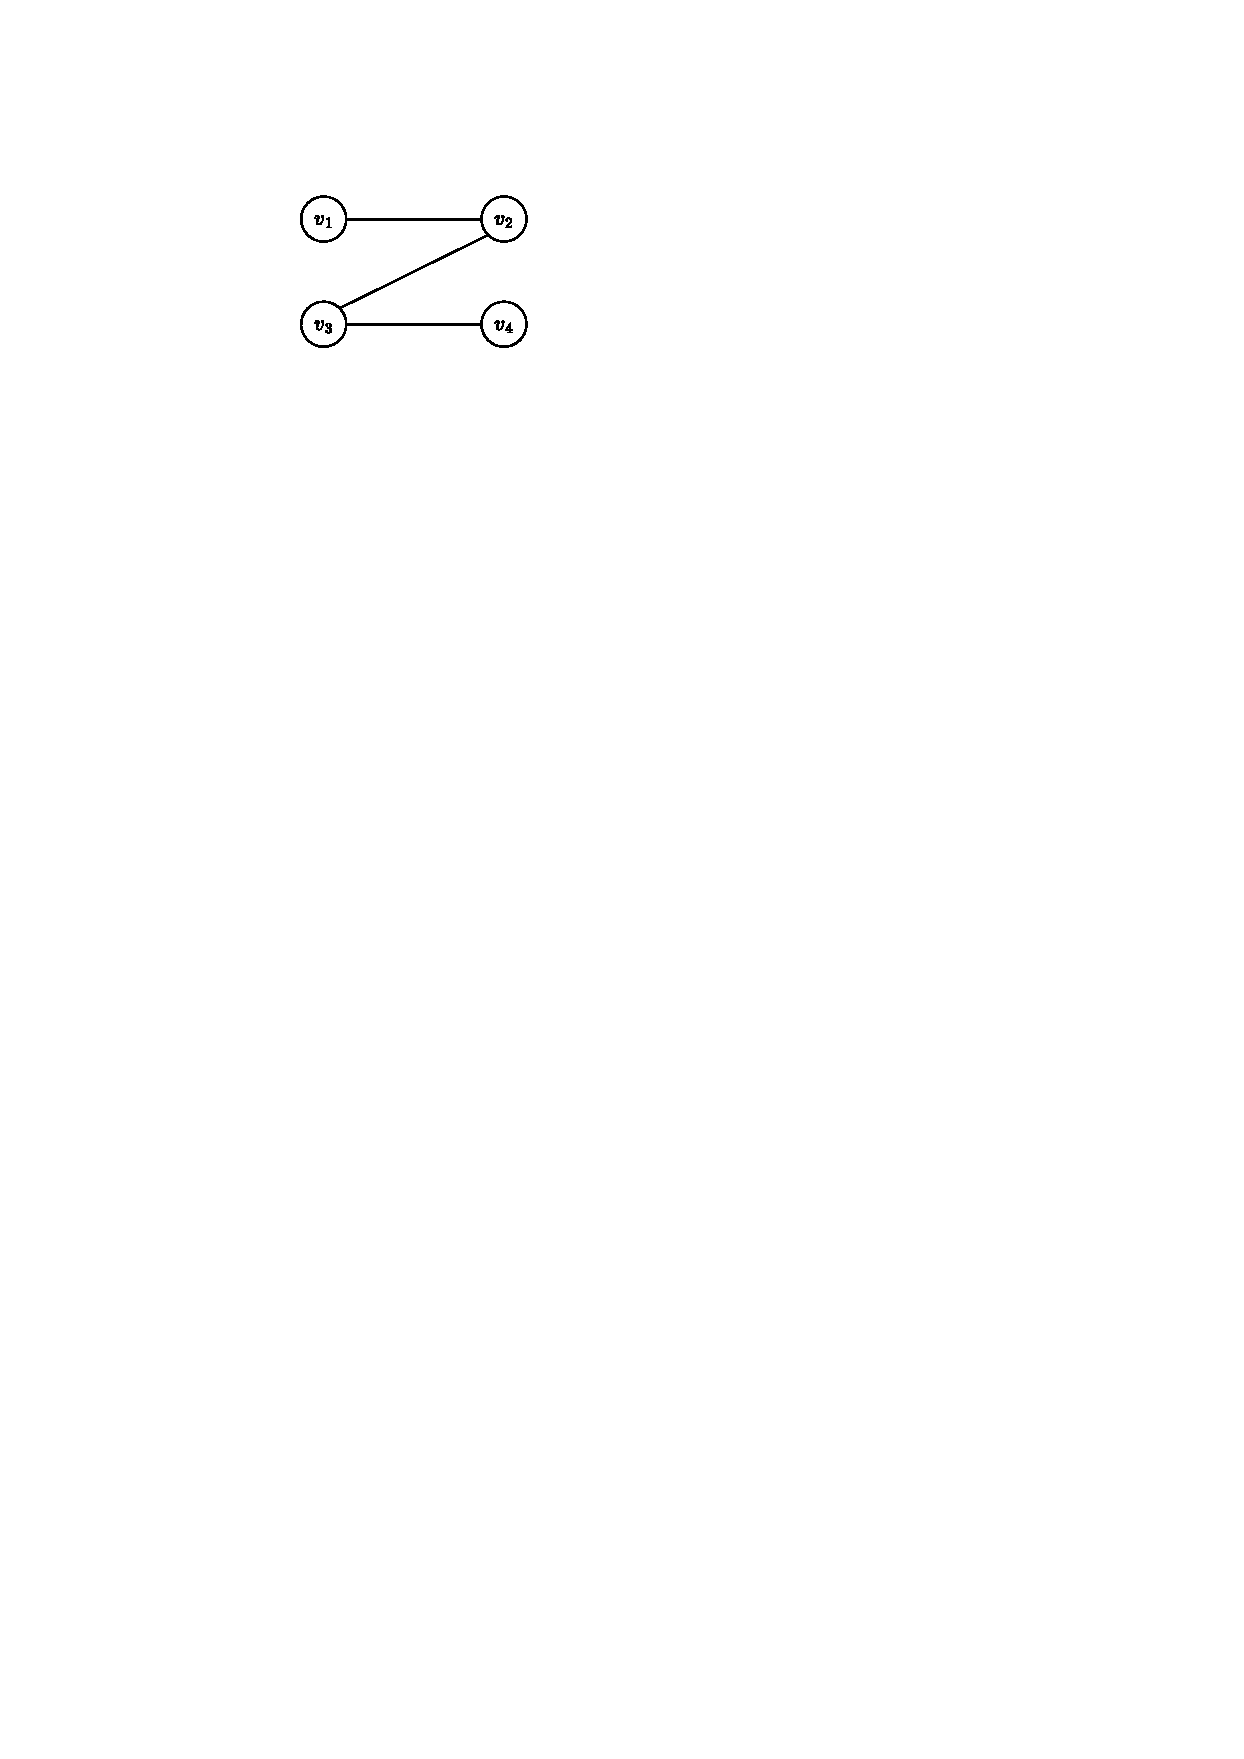
\includegraphics[width=5cm]{images/matching.pdf}
    \end{center}
    \caption{マッチング$M_1=\{v_1,v_2\},\{v_3,v_4\}\}$と$M_2=\{\{v_2,v_3\}\}$はどちらも極大である. \label{fig:matching}}
\end{figure}

\paragraph*{例6.}
グラフ$G=(V,E)$の頂点部分集合$U\subseteq V$は, $U$に属する任意の二頂点間に辺がある(すなわち$\binom{U}{2}\subseteq E$)とき, \emph{クリーク (clique)}\footnote{cliqueとは派閥を意味する英単語である.}という.
特に, 単一頂点からなる集合$\{u\}$や$\emptyset$もクリークである.
クリークの部分集合もまたクリークなので,
グラフ$G$の全てのクリークからなる頂点集合族を$\F$とすると, $(V,\F)$は単体複体である.

\begin{definition}{リンクとスケルトン}{link and skelton}
    単体複体$X=(V,\F)$を考える.
    面$\sigma \in \F$の\emph{リンク (link)}とは単体複体$(V\setminus \sigma, \F_{\sigma})$であって集合族$\F_\sigma$が
    \[
        \F_\sigma = \cbra*{ \tau \setminus \sigma \colon \sigma \subseteq \tau \in \F }
    \]
    で与えられるものである.
    次元$k$以下の面の集合
    \[
        \F_k = \cbra*{ \sigma \in \F \colon \dim \sigma \le k}
    \]
    に対し$(V,\F_k)$を\emph{$k$-スケルトン ($k$-skelton)}という.
\end{definition}
面$\sigma$のリンクとは, $\sigma$をある意味で「縮約」して得られる単体複体であり, 面$\sigma$の周りの局所的な構造を表している.
例えば連結グラフ$G=(V,E)$の森の全体からなる単体複体$X=(E,\F)$を考えよう.
$\sigma\in \F$を一つ固定したとき, リンク$X_\sigma$はどのような単体複体になっているだろうか?
$X_\sigma$の全ての面は辺集合$F$を含むので, $F$に含まれる全ての頂点を縮約して得られるより小さなグラフを考え, そこから$F$の辺を除去して得られるグラフ$G'$の森全体からなる単体複体とみなせる.

%\end{definition}
\section{大域エクスパンダー性}
グラフ上のランダムウォークは頂点集合上で遷移するものを考えていたが,
単体グラフ上のランダムウォークは異なる次元の面の間で遷移するものを考える.
具体的には, \cref{sec:graph up and down walk}で考えたようにある次元$i$の面から次元$i+1$の面に遷移する上昇ウォークと逆に次元$i+1$の面から次元$i$の面に遷移する下降ウォークである.
上昇ウォークと下降ウォークが互いに随伴の関係になるようにするため, 各$X(i)$上での定常分布を定義し, $X(i)$と$X(i+1)$の間で詳細釣り合い条件が満たされるように定義される.

\subsection{下降ウォークと定常分布}
まず, \cref{sec:graph up and down walk}で考えた下降ウォークを単体複体に拡張し, $X(d-1)$上では一様分布を定常分布とすることによって帰納的に各$X(i)$上での定常分布を定める.
\begin{definition}{下降ウォークと面上の定常分布}{down walk and stationary distribution}
    純粋な$d$次単体複体$X=(V,\F)$を考える.
    各$i=0,\dots,d-1$に対し
        確率行列$\Pdown_i \in [0,1]^{X(i) \times X(i-1)}$を
        \[
            \Pdown_i(\tau,\sigma) = \begin{cases}
                \frac{1}{i+1}	& \tif \sigma \subseteq \tau,\\
                0 & \totherwise
            \end{cases}
        \]
        とする.
    各$i=0,\dots,d-1$に対して, $X(i)$上の分布$\pi_i \in [0,1]^{X(i)}$を
        \begin{itemize}
        \item $i=d-1$のとき, $\pi_{d-1}$は$X(d-1)$上の一様分布. すなわち$\pi_{d-1}(\sigma) = \frac{1}{\abs{X(d-1)}}$
        \item $\pi_{i+1}$が定義されているとき, $\pi_i = \pi_{i+1}\Pdown_{i+1}$
        \end{itemize}
    で定める.
    分布$\pi_i$を($i$次の)定常分布と呼ぶ.
\end{definition}
面$\tau \in X(i+1)$に対して$\Pdown_{i+1}(\tau,\cdot)$で定まる$X(i)$上の分布は, 面$\tau$に含まれる頂点$u$を一様ランダムに選んだときの$\sigma = \tau \setminus\{u\}$の分布と等しい.
この分布は, まず一様ランダムに$X(d)$から面を選び, その中から一様ランダムに選ばれた$i+1$個の頂点からなる$X(i)$の面のなす分布である.
特に全ての$\sigma\in X(i)$に対し$\pi_i(\sigma)=0$である
(そうでなければ, $\pi_d$が一様分布であることに反する).
ある面$\tau\in X(i+1)$から分布$\Pdown_{i+1}(\tau,\cdot)$に従ってランダムに選ばれた面$\sigma$に遷移する過程を\emph{下降ウォーク (down walk)}と呼ぶ.

\subsection{上昇ウォーク}
\cref{def:down walk and stationary distribution}では次元$i$の面から次元$i-1$に遷移する下降ウォークを与えた.
同様に, 次元$i$の面から次元$i+1$の面に遷移する上昇ウォークを, $X(i)$と$X(i+1)$の間の詳細釣り合い条件が成り立つように定義する.
%
\begin{definition}{上昇ウォーク}{up walk}
    純粋な$d$次単体複体$X=(V,\F)$を考える.
    各$i=-1,\dots,d-2$に対し
        確率行列$\Pup_i \in [0,1]^{X(i) \times X(i+1)}$を
    \begin{align*}
        \Pup_i(\sigma,\tau) &= \frac{\pi_{i+1}(\tau)}{\pi_i(\sigma)}\Pdown_{i+1}(\tau,\sigma) \\
        &= \begin{cases}
            \frac{\pi_{i+1}(\tau)}{(i+1)\pi_i(\sigma)}	& \tif \sigma\subseteq \tau,\\
            0 & \totherwise
        \end{cases}
    \end{align*}
    で定める.
\end{definition}
%
二つの面集合$X(i)$と$X(i+1)$を部集合とする二部グラフを考えればわかりやすい.
それぞれの部集合には$\pi_i,\pi_{i+1}$が定常分布として付随しており,
上昇ウォーク$\Pup_i$と下降ウォーク$\Pdown_{i+1}$は詳細釣り合い条件
\[
    \forall \sigma\in X(i),\tau\in X(i+1),\,\pi_i(\sigma)\Pup_i(\sigma,\tau) = \pi_{i+1}(\tau)\Pdown_{i+1}(\tau,\sigma)
\]
を満たしている.

なお, 下降ウォーク$\Pdown_{i}$と上昇ウォーク$\Pup_i$の添字$i$は遷移の開始地点の面の次元としている.
%
    各$X(i)$に対して空間$\ell^2_{\pi_i}(X(i))$, 
    すなわち, \cref{def:naiseki}と同様にして$\Real^{X(i)}$に内積$\abra{\cdot,\cdot}_{\pi_i}$が導入された空間を定義できる.
    このとき, 
    \[\Pup_i\colon \ell^2_{\pi_{i+1}}(X(i+1)) \to \ell^2_{\pi_{i}}(X(i))\]
    と
    \[\Pdown_{i+1}\colon \ell^2_{\pi_{i}}(X(i)) \to \ell^2_{\pi_{i+1}}(X(i+1))\]
    は互いに随伴の関係にある.
    すなわち, 任意の$f\in \ell^2_{\pi_i}(X(i)),g\in \ell^2_{\pi_{i+1}}(X(i+1))$に対して
    \begin{align} \abra{\Pup_i f, g}_{\pi_{i+1}} = \abra{ f,\Pdown_{i+1}g }_{\pi_i} \label{eq:adjoint up and walk}\end{align}
    が成り立つ.
%
\begin{exercise}{}{adjoint check}
    \cref{eq:adjoint up and walk}を確認せよ.
    すなわち, \cref{def:down walk and stationary distribution}で定義された定常分布$\pi_i,\pi_{i+1}$および任意の二つの関数$f\colon X(i) \to \Real,g\colon X(i+1) \to \Real$に対して
    \[ \sum_{\sigma \in X(i)} \pi_i(\sigma) f(u) = \sum_{\tau \in X(i+1)} \pi_{i+1}(\tau) g(\tau) \]
を確認せよ.
\end{exercise}

最後に, 上昇ウォークと下降ウォークを組み合わせることによって面$X(i)$上の2種類のランダムウォークが定義できる:
\begin{definition}{上昇下降と下降上昇ウォーク}{UD and DU walk}
    \cref{def:down walk and stationary distribution}, \ref{def:up walk}と同じ設定を考える.
    \begin{align*}
        &\PUD_i \defeq  \Pup_i \Pdown_{i+1},\\
        &\PDU_i \defeq \Pdown_{i}\Pup_{i-1}
    \end{align*}
    を遷移確率行列として持つ$X(i)$上のランダムウォークをそれぞれ\emph{上昇下降ウォーク (up-down walk), 下降上昇ウォーク (down-up walk)}と呼ぶ.
    ここで, $X(-1)$上での下降上昇ウォークと$X(d-1)$上での上昇下降ウォークは定義されない.
\end{definition}
上昇下降ウォークはグラフ上の遅延単純ランダムウォークの自然な一般化になっている (\cref{sec:graph up and down walk}).
\begin{lemma}{定常分布}{UP and DU stationary distribution}
    面$X(i)$上の上昇下降ウォークと下降上昇ウォークはどちらも$\pi_i$を定常分布としてもつ.
\end{lemma}
\begin{proof}
    計算によって簡単に確認できる.
    実際,
    \begin{align*}
        &\pi_i \PUD_i = \pi_i \Pup_i \Pdown_{i+1} = \pi_{i+1} \Pdown_{i+1} = \pi_i, \\
        &\pi_i \PDU_i = \pi_i \Pdown_i \Pup_{i-1} = \pi_{i-1}\Pup_{i-1} = \pi_i
    \end{align*}
    より主張を得る.
\end{proof}
\begin{remark}{「上昇」「下降」の名称}{up and down}
    非常にややこしいのだが,
    上昇ウォークと下降ウォークの遷移確率行列と左右どちらから作用させるかによって「上昇」「下降」の意味合いが反転してしまう.
    確率行列としての上昇ウォークは$\Pup_i \in [0,1]^{X(i)\times X(i+1)}$で表せる.
    一般によくある左から作用させる作用素の感覚で考えると
    $\Pup_i\colon \Real^{X(i+1)} \to \Real^{X(i)}$
    であるので, 次元を一つ落とすように見えてしまうのである.
    下降ウォークについても同様である.
    特に上昇下降ウォーク$\PUD_i=\Pup_i\Pdown_{i+1}$を左から作用させると「次元を下げてから上げる」ものになるので, 下降上昇ウォークと混同しやすい.
    
    本講義はランダムウォークを主眼におき, 右から作用させるときの$\Pup_i,\Pdown_i$に興味があるので, 左固有値以外の文脈ではとにかくランダムウォークの遷移確率行列といえば右から作用させるものであると考えていき, 名称についても
    \cref{def:down walk and stationary distribution}, \ref{def:up walk}の呼称を採用している.
    
    そもそも, 遷移確率行列$P(u,v)$を「$u$から$v$に遷移する確率」として定義してしまったのが根本的な原因であり, 転置したものを改めて遷移確率行列と定義しなおせば解決できるのだが, ランダムウォークの文化ではもはや\cref{def:random walk}の定義が完全に主流となってしまっておりそれに反するとほとんどの参考文献が読みづらくなってしまうので従った.
    
    なお, 可逆なランダムウォーク(\cref{def:reversible})は内積$\piprod{\cdot,\cdot}$の意味で左右どちらから作用させても本質的に同じであるので左右どちらから作用させるかについてこのような煩雑な話は考えなくて良い.
\end{remark}

\section{局所エクスパンダー性}
単体複体の各リンクに対して局所的なランダムウォークを次のように定義する.
\subsection{局所的なランダムウォーク}
全てのリンクの$2$-スケルトン上での局所的な重み付きランダムウォークを考える.
重み付きランダムウォークについては\cref{def:weighted random walk}を参照されたい.
%
\begin{definition}{局所ランダムウォーク}{local random walk}
    純粋な$d$次元単体複体$X = (V,\F)$を考える.
    次元$i \le d-2$の面$\sigma \in \F$に対し,
        リンク$X_\sigma$の$2$-スケルトンを$G_\sigma = (V_\sigma,E_\sigma)$とする.
    このグラフの辺重み$w_\sigma\colon E_\sigma \to [0,1]$を
    \[ w_\sigma(e) = \pi_i(\sigma\cup e) \]
    で定め, これによって定まる$V_\sigma$上の重み付きランダムウォークを面$\sigma$に関する\emph{局所ランダムウォーク (local random walk)}と呼び\footnote{このランダムウォークの概念は高次元エクスパンダーの文脈ではほぼ必ず登場するが, 特に標準的な用語が与えられてはいないので、「局所ランダムウォーク」という用語は本講義だけの局所的なものとする.}, 遷移確率行列を$P_\sigma\in [0,1]^{V_\sigma\times V_\sigma}$とする.
\end{definition}
%
必ずしも局所ランダムウォークが既約性や非周期性を持つとは限らない(すなわち, グラフ$G_\sigma$が非連結だったり二部グラフになりうる)が,
可逆性は必ず満たすことに注意せよ.

グラフ($1$次元単体複体)だと面$\emptyset$に対する局所ランダムウォークのみ存在するが, これは上昇下降ウォーク(すなわち遅延単純ランダムウォーク)と同じである.
従って局所ランダムウォークの概念はより高次元の単体複体を考える際に意味を持つ.

%
\begin{lemma}{}{local random walk stationary distribution}
    遷移確率行列$P_\sigma$をもつ局所ランダムウォークの定常分布を$\pi_\sigma$とすると, 
\end{lemma}
%
\subsection{局所エクスパンダー}
純粋な単体複体の局所的なエクスパンダー性を定義する.
任意の面$\sigma$に対し$G_\sigma$上での局所ランダムウォークの第二固有値が小さいとき, その単体複体は局所的エクスパンダー性をもつという.
\begin{definition}{局所エクスパンダー性}{local expander}
    純粋な$d$次元単体複体$X=(V,\F)$は,
    任意の面$\sigma\in\F$に対し$\lambda_2(P)\le \lambda$を満たすとき,
    \emph{局所$\lambda$-エクスパンダー (local $\lambda$-expander)}であるという.
    より一般に, 任意の$i=-1,\dots,d-2$と任意の面$\sigma\in X(i)$に対して$\lambda_2(P_\sigma) \le \lambda_i$を満たすとき, 単体複体$X$は局所$(\lambda_{-1},\dots,\lambda_{d-2})$-エクスパンダーであるという.
\end{definition}
エクスパンダーグラフ(\cref{def:expander})と比較すると, 片側($\lambda_2$)だけの上界だけでエクスパンダー性を定義している.
これは, 単体複体上の上昇下降ウォークがグラフ上の遅延単純ランダムウォークに対応していることに起因する (遅延単純ランダムウォークの遷移確率行列は半正定値だから$\lambda_2$の上界だけあれば混交性が保証される).
%

\section{Oppenheimのトリクルダウン定理}

\section{高次元エクスパンダーの応用}
理論計算機科学における高次元エクスパンダーの応用を簡単にまとめる.
特にマトロイドに関するものは次チャプターにて解説する.
本質的には,
局所的な情報(局所ランダムウォークの混交性)が大域的な情報(上昇下降ランダムウォークの混交性)を導出するという性質が極めて重要であり,
これに基づいて誤り訂正符号などの構成がなされている.
\chapter{マトロイド} \label{chap:matroid}
マトロイド(matroid)は「行列(matrix)のようなもの(-oid)」という名を冠するが,
線形代数における線型独立性をグラフの全域木などに拡張した概念である.

\section{定義}
\begin{definition}{マトロイド}{matroid}
    次の性質を持つ単体複体$(V,\F)$を\emph{マトロイド (matroid)}という:
    任意の$\sigma,\tau \in \F$に対し, $\abs{\sigma} < \abs{\tau}$ならば,
    ある$ u \in \tau \setminus \sigma$が存在して
    $\sigma \cup \cbra{u} \in \F$.

    マトロイド$(V,\F)$の面$\sigma\in \F$を特に\emph{独立集合 (independent set)}という.
\end{definition}

\begin{definition}{基}{basis}
    マトロイドの(包含関係に関して)極大な独立集合を\emph{基 (basis)}といい, 基全体の集合を$\B$で表す.
    特に断りのない限り, 基上の定常分布は一様分布とする.
\end{definition}
マトロイドは純粋な単体複体である.
実際, もし$\abs{B} < \abs{B'}$なる二つの基$B,B'\in\B$が存在するならば,
マトロイドの定義(\cref{def:matroid})より,
ある$u \in B'\setminus B$が存在して$B\cup \{u\} \in \F$とできるが,
これは$B$の極大性に矛盾する.

\paragraph*{例1. 一様マトロイド}
\cref{eq:uniform matroid}で定まる単体複体$(V,\F)$は\emph{一様マトロイド (uniform matroid)}と呼ばれるマトロイドである.

\paragraph*{例2. グラフ的マトロイド}
\cref{eq:graphic matroid}で定まる単体複体$(V,\F)$はマトロイドである.
ここでは証明の概要を説明する.
マトロイドであることを示すには, 任意の二つの森$\sigma,\tau \in \F,\abs{\sigma} < \abs{\tau}$に対して, ある辺$e\in \tau\setminus \sigma$が存在して$\sigma\cup\{e\}$が閉路を含まないようにできることを言えばよい.
二つの森$\sigma,\tau \in \F,\abs{\sigma} < \abs{\tau}$を固定する.
森$\sigma\in \F$はグラフ上で複数の連結成分をなす.
これら連結成分の個数は$|V| - \abs{\sigma}$に等しい.
さて, 森$\tau$の中には, $\sigma$のなす連結成分のうち相異なる二つの間を横切る辺$e \in \tau \setminus \sigma$が存在する (\cref{fig:graphicmatroid}).
そうでなければ, $\tau$のなす連結成分の個数$|V|-\abs{\tau}$は$|V|-\abs{\sigma}$以下となってしまい, $\abs{\tau} > \abs{\sigma}$に矛盾.
この辺$e$を$\sigma$に追加しても閉路は発生しない.
(もし閉路$C$が生じるならば, $e$が$\sigma$のなす連結成分を横切ることに矛盾する).
すなわち, $\sigma\cup\{e\}\in\F$であり, 確かに$(V,\F)$はマトロイドである.
%
\begin{figure}
    \begin{center}
    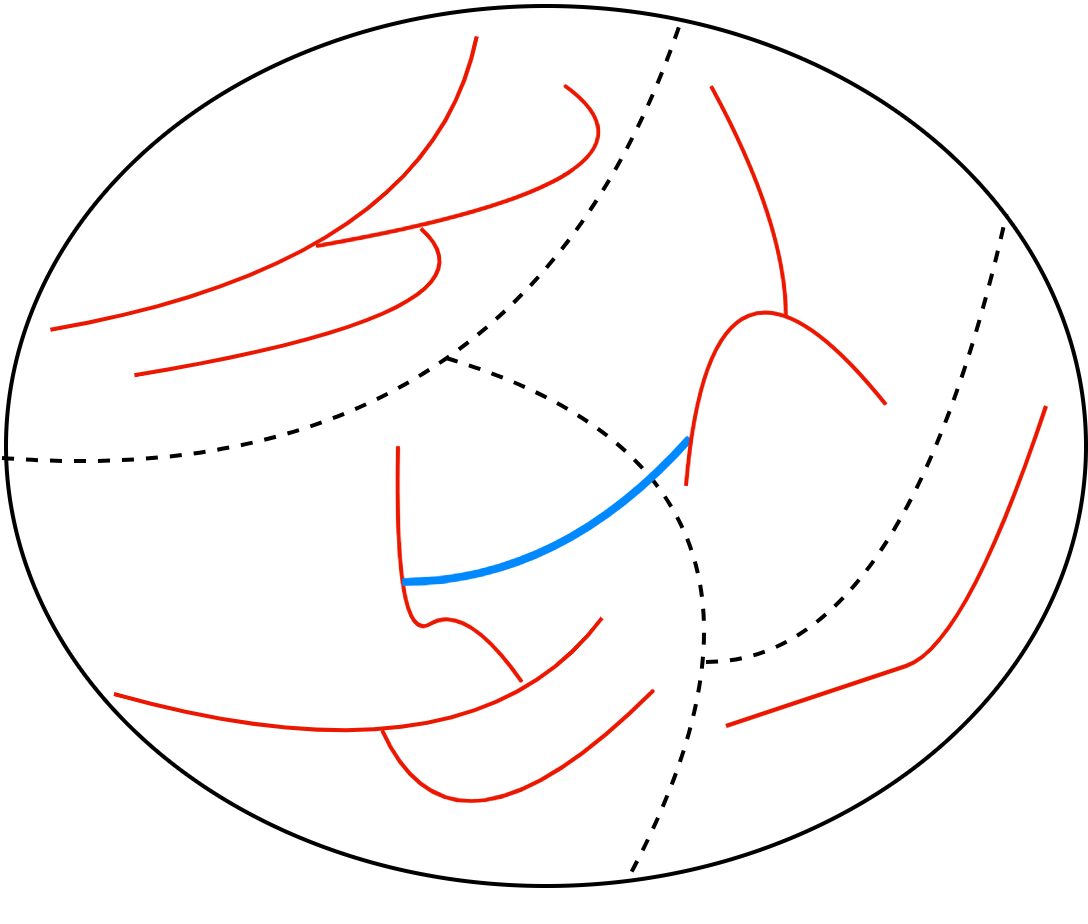
\includegraphics[width=7cm]{images/graphicmatroid.png}
    \caption{森$\sigma$のなす連結成分をまたがる辺$e \in \tau$が必ず存在する. \label{fig:graphicmatroid}}
    \end{center}
\end{figure}

グラフの森から定まる上記のマトロイドは\emph{グラフ的マトロイド (graphic matroid)}と呼ばれるマトロイドの重要なクラスをなす.

%
\paragraph*{例3. 線形マトロイド}
\cref{eq:linear matroid}で定まる単体複体$(V,\F)$は\emph{線形マトロイド (linear matroid)}と呼ばれるマトロイドである.

\paragraph*{例4. 分割マトロイド}
有限集合$V$の分割$V=W_1\sqcup \dots \sqcup W_k$と非負整数$d_1,\dots,d_k\ge 0$を固定する.
部分集合族$\F$を
\begin{align}
    F \in \F \iff \forall i\in\{1,\dots,k\},\abs{W \cap W_i} \le d_i     \label{eq:partition matroid}
\end{align}
で定義したとき, $(V,\F)$は\emph{分割マトロイド (partition matroid)}と呼ばれるマトロイドである.
平たく言えば, 各$W_i$の元を高々$d_i$個ずつ含むものからなる部分集合族である.

\begin{exercise}{}{partition matroid}
    \cref{eq:partition matroid}で定まる単体複体$(V,\F)$がマトロイドであることを示せ.
\end{exercise}

\paragraph*{マトロイドでない例.}
クリーク複体やマッチング全体のなす単体複体はそもそも純粋とは限らないので必ずしもマトロイドになるとは限らない.

\section{基交換ウォーク}
\begin{definition}{基交換ウォーク}{basis-exchange walk}
    マトロイド$(V,\F)$の基上の下降上昇ウォークを\emph{基交換ウォーク (basis-exchange walk)}という.
\end{definition}
すなわち, 基$B$から開始し,
一様ランダムに元$u\sim B$を選び,
$B\setminus u$を含む基の中から一様ランダムな基$B'\in B'$に遷移するランダムウォークを基交換ウォークという (このとき定常分布は$\B$上の一様分布となる).
基交換ウォークの混交時間のバウンドは長年の未解決問題であった.
\begin{conjecture}{Mihail--Vazirani予想}{Mihail-Vazirani}
    任意のマトロイド$M=(V,\F)$上の基交換ウォークの混交時間は$|V|$に関する多項式で上から抑えられる.
    すなわち, $M$に依存しないある定数$c>0$が存在して
    \[
        \tmix(1/2) \le |V|^c.
    \]
\end{conjecture}
基全体の個数は$\abs{V}$に関して指数関数的であるが,
ここでは
\emph{多項式ステップ}の基交換ウォークで混ざり合うかを問うている.
グラフ的マトロイドといった特殊ケースでは\cref{conj:Mihail-Vazirani}が正しいことが知られていた
\cite{balanced_matroids}が, 一般のマトロイドで正しいかどうかは未解決であった.

\section{マトロイドの局所エクスパンダー性}
本節では以下の定理を証明する.
\begin{lemma}{}{local expander matroid}
    任意のマトロイド$(V,\F)$は局所$0$-エクスパンダーである.
\end{lemma}


\subsection{Oppenheimのトリクルダウン定理}
ある単体複体$X$に対して局所エクスパンダー性(\cref{def:local expander})を示すには全ての面に対して$\lambda_2(P_\sigma)$を上から抑える必要がある.
一般にそもそも辺重み$w_\sigma$ (\cref{def:local random walk}) を求めることすら非自明であり, ましてや固有値を抑えるなど非常に大変な作業となる.
Oppenheimのトリクルダウン定理は局所エクスパンダー性を確認するのに非常に有用な定理である.
\begin{theorem}{Oppenheimのトリクルダウン定理}{Oppenheim trickle-down theorem}
    純粋な重み付き$d$-次元単体複体$X = (V,\F)$が以下の二つを満たすとする:
    \begin{itemize}
    \item 全ての$i\le d-2$と全ての$\sigma\in X(i)$に対してグラフ$G_\sigma$は連結.
    \item 全ての$(d-2)$-次元の面$\tau \in X(d-2)$に対して$\lambda_2(P_\tau) \le \gamma$.
    \end{itemize}
    このとき, $\gamma_i \defeq \frac{\gamma}{1-(d-2-i)\gamma}$ ($i=-1,\dots,d-2$)に対して$X$は局所$(\gamma_{-1},\dots,\gamma_{d-2})$-エクスパンダーである.
\end{theorem}
端的に言えば, 次数$d-2$の面$\sigma \in X(d-2)$に対して$\lambda(P_\sigma)$を抑えれば全ての次元の面に対しても第二固有値が上から抑えられるという結果である.

一つ目のグラフ$G_\sigma$の連結性の条件は不可欠である.
例えば二つの完全グラフからなる非連結グラフ上の三角形複体を考えると,
空集合以外の全てのリンクは完全グラフ上のランダムウォークとなるため$\gamma=0$に対して二つ目の条件を満たすが, $\sigma=\emptyset$に対して$G_\sigma$は非連結であるため$\gamma_{-1}=0$にはならない.


\cref{thm:Oppenheim trickle-down theorem}は, まず$d=2$の特殊ケースで証明し, 一般の$d$についてはこの特殊ケースに帰着する.
%
\begin{lemma}{\texorpdfstring{$d=2$}{2次元}におけるトリクルダウン定理}{trickle-down for 2dim}
    純粋な重み付き$2$次元単体複体$X=(V,\F)$の各頂点$v\in X(0)$における局所ランダムウォーク$P_v$が$\lambda_2(P_v) \le \gamma$を満たし, かつその$1$-スケルトン$G_v$が連結ならば, 面$\emptyset$における局所ランダムウォーク$P_\emptyset$は
    \[
        \lambda_2(P_\emptyset) \le \frac{\gamma}{1-\gamma}
    \]
    を満たす.
\end{lemma}
\subsection{ランダムウォークの分解}
\cref{lem:trickle-down for 2dim}の証明は,
\cref{thm:Kaufman-Oppenheim theorem}と同様にランダムウォークを分解することから始まる.
記法の簡単のため, 頂点$u$のリンクを$X_{\{u\}}$の代わりに$X_u$, 遷移確率行列を$P_{\{u\}}$の代わりに$P_u$と表す.
\begin{definition}{}{localize}
    重み付き単体複体$(V,\F)$, 頂点$u\in V$, 関数$f \in \ispace[X(0)]$に対し,
    関数$f^u \in \ispace[X_u(0)]$を$f$の$X_u(0)$への制限, すなわち
    \[
        f^u (v) = f(v)
    \]
    とする.
\end{definition}
簡単な計算から以下の二次形式の分解補題が成り立つことがわかる.
\begin{lemma}{}{decomposition}
    任意の$f,g\in \ispace[X(0)]$に対して
    \[
        \iprod[X(0)]{f,g} = \E_{u\sim X(0)}\sbra*{ \iprod[X_u(0)]{f^u,g^u} }.
    \]
    また, 面$\emptyset$上の局所ランダムウォークの遷移確率行列を$P_\emptyset \in [0,1]^{X(0)\times X(0)}$とすると,
    \[
        \iprod[X(0)]{P_\emptyset f,g} = \E_{w\sim X(0)}\sbra*{ \iprod[X_u(0)]{P_uf^u,g^u} }.
    \]
\end{lemma}
\begin{proof}
    最初の等式を示す:
    \begin{align*}
        (\text{左辺}) &= \E_{u\sim X(0)} \sbra*{ f(u) g(u) } \\
        &= \E_{e \sim X(1)}\sbra*{ \E_{v \sim e} \sbra*{f(v)g(v)}} & & \text{$v\sim e$の周辺分布は$\pi_0$}\\
        &= \E_{u\sim X(0)} \sbra*{ \E_{\substack{e=\{u,v\} \sim X(1) \\ \text{conditioned on }e\ni u} }\sbra*{ f(v)g(v) }} & & \text{$e\sim X(1)$の$v$でない方の端点$u$を先に選ぶ}\\
        &= \E_{u\sim X(0)}\sbra*{ \E_{v \sim X_u(0)} \sbra*{f^u(v) g^u(v)} } & & \text{$\because$\cref{rem:link of u}}\\
        &= (\text{右辺}).
    \end{align*}
    二つ目の等式を示す.
    \begin{align*}
        (\text{左辺}) &= \E_{\{u,v\} \sim X(1)}\sbra*{f(u)g(v)} \\
        &= \E_{t \sim X(1)}\sbra*{ \E_{\substack{w \sim t \\ \{u,v\} = t\setminus w}} \sbra*{f(u)g(v)} } \\
        &= \E_{w\sim X(0)}\sbra*{ \E_{\substack{t \sim X(2) \\ \text{conditioned on }t \ni w \\ \{u,v\}= t \setminus w}} \sbra*{f(u)g(v)} } & & \text{前式の$w$の周辺分布は$X(0)$}\\
        &= \E_{w\sim X(0)}\sbra*{ \E_{\{u,v\}\sim X_w(1)}\sbra*{f(u)g(v)} } \\
        &= (\text{右辺}).
    \end{align*}
\end{proof}
%
\begin{proof}[\textbf{\cref{lem:trickle-down for 2dim}の証明.}]
    記号の簡単のため$P=P_\emptyset$とする.
    局所ランダムウォーク$P$の第二固有値に対応する固有ベクトルを$f$とする.
    正規化して$\inorm[X(0)]{f}=1$とする.
    $P_\emptyset$の可逆性および\cref{lem:Rayleigh quotient}から,
    $\iprod[X(0)]{f,\allone}=0$である.
    補題を証明するには, $ \lambda_2(P)=\iprod[X(0)]{P f,f}$を上から抑えればよい.

    各頂点$u \in X(0)$に対し\cref{def:localize}で定義された$f^u \in \ispace[X_u(0)]$を考える.
    このベクトルを直交分解し,
    \begin{align}
        f^u = \alpha_u \allone^u + \overline{f^u} \label{eq:eigen decomposition fu}
    \end{align}
    と表す.
    ここで, $\allone^u \in \ispace[X_u(0)]$は全成分が$1$のベクトルで, $\alpha_u=\iprod[X_u(0)]{f,\allone^u}$であり, $\overline{f^u}$は$\allone^u$に直交するベクトルである.

    直交分解(\ref{eq:eigen decomposition fu})を用いると
    \begin{align*}
        \iprod[X_u(0)]{P_u f^u,f^u} &= \iprod[X_u(0)]{P_u\rbra*{\alpha_u\allone^u + \overline{f^u}}, \alpha_u\allone^u+\overline{f^u}} \\
        &= \iprod[X_u(0)]{\alpha_u \allone^u + P_u\overline{f^u}, \alpha_u\allone^u+\overline{f^u}} \\
        &= \alpha_u^2 + \iprod[X_u(0)]{P_u\overline{f^u},\overline{f^u}}  & & \text{直交性よりクロスタームは消える}\\
        &\le \alpha_u^2 + \gamma\inorm[X_u(0)]{\overline{f^u}}^2 & & \text{$\because$$\lambda_2(P_u)\le \gamma$および\cref{lem:Rayleigh quotient}}
    \end{align*}
    を得る.
    \cref{lem:decomposition}より,
    \begin{align*}
        \lambda_2(P) &= \iprod[X(0)]{Pf,f} \\
        &= \E_{u\sim X(0)}\sbra*{ \iprod[X_u(0)]{P_u f^u,f^u} } & & \text{$\because$\cref{lem:decomposition}の二つ目の等式} \\
        &\le \E_{u\sim X(0)}\sbra*{\alpha_u^2} + \gamma\cdot \E_{u\sim X(0)}\sbra*{\inorm[X_u(0)]{\overline{f^u}}^2} & & \text{直前の不等式を代入}\\
        &= \gamma\cdot \E_{u\sim X(0)}\sbra*{\alpha_u^2 + \inorm[X_u(0)]{\overline{f^u}}^2} + (1-\gamma)\cdot \E_{u\sim X(0)}\sbra*{\alpha_u^2} \\
        &= \gamma\cdot \E_{u\sim X(0)}\sbra*{\inorm[X_u(0)]{f^u}^2} + (1-\gamma)\cdot \E_{u\sim X(0)}\sbra*{\alpha_u^2} & & \text{$\because$$f^u$に対する三平方の定理}\\
        &= \gamma \cdot \inorm[X(0)]{f}^2 + (1-\gamma)\cdot \E_{u\sim X(0)}\sbra*{\alpha_u^2} & & \text{$\because$\cref{lem:decomposition}を$\iprod[X(0)]{f,f}$に適用} \\
        &= \gamma + (1-\gamma)\cdot \E_{u\sim X(0)}\sbra*{\alpha_u^2} & & \text{$f$のノルムは$1$}
    \end{align*}
    を得る.
    従って, $\E_{u\sim X(0)}\sbra*{\alpha_u^2}$を上から抑えたい.

    内積$\iprod[X_u(0)]{\cdot,\cdot}$の定義から
    \begin{align*}
        \alpha_u &= \iprod[X_u(0)]{f^u,\allone^u} \\
        &= \E_{v \sim X_u(0)}\sbra*{f^u(v)} \\
        &= \E_{v \sim X_u(0)}\sbra*{ f(v) } & & \text{\cref{def:localize}参照}\\
        &= (Pf)(u) & & \text{$P=P_\emptyset$は$1$-スケルトン上のランダムウォーク}
    \end{align*}
    であり, $f$は$P$の固有ベクトルなので
    \begin{align*}
        \E_{u\sim X(0)}\sbra*{\alpha_u^2} &= \inorm[X(0)]{Pf}^2 = \lambda_2(P)^2.
    \end{align*}
    これを代入すると二次不等式
    \begin{align*}
        \lambda_2(P) \le \gamma + (1-\gamma)\lambda_2(P)^2
    \end{align*}
    を得る. これを$\lambda_2(P)$について解くと
    \[
     \lambda_2(P)\ge 1 \text{ または }\lambda_2(P) \le \frac{\gamma}{1-\gamma}
    \]
    となるが, $1$-スケルトン$G_v$の連結性の仮定より$\lambda_2(P)<1$なので, $\lambda_2(P) \le \frac{\gamma}{1-\gamma}$を得る.    
\end{proof}
%
\subsection{トリクルダウン定理の証明}
\cref{lem:trickle-down for 2dim}を用いて一般の次元$d$に対する\cref{thm:Oppenheim trickle-down theorem}を証明する.
%
\begin{proof}[\textbf{\cref{thm:Oppenheim trickle-down theorem}の証明.}]
    $X=(V,\F)$を純粋な重み付き$d$次元単体複体とする ($d\ge 3$).
    面$\sigma \in X(d-3)$のリンク$X_\sigma$の次元は$2$であり,
    $X_\sigma$の頂点$v\in X_\sigma(0)$に対して
    $\sigma \cup \{v\} \in X(d-2)$より,
    $X_\sigma$上の$v$における局所ランダムウォークの遷移確率行列は$P_{\sigma\cup \{v\}}$に等しく, 仮定より$\lambda_2\rbra*{P_{\sigma\cup\{v\}}}\le \gamma$である.
    さらに, $X$の各リンクの$1$-スケルトンは連結なので, \cref{lem:trickle-down for 2dim}より
    \[
        \lambda_2(P_\sigma) \le \frac{\gamma}{1-\gamma}
    \]
    を得る.
    同じ議論を, $X$をその$(d-1)$-スケルトンに置き換えて適用すると,
    任意の$\sigma' \in X(d-4)$に対し
    \[
        \lambda_2(P_{\sigma'}) \le \frac{\frac{\gamma}{1-\gamma}}{1- \frac{\gamma}{1-\gamma}} = \frac{\gamma}{1-2\gamma}
    \]
    を得る.
    これを繰り返すと, ($j$に関する帰納法により)
    面$\rho \in X(d-2-j)$に対し
    \[
        \lambda_2(P_\rho) \le \frac{\gamma}{1-j\gamma}
    \]
    を得る.
\end{proof}
%


\section{Anari, Liu, Gharan, Vinzantの定理}
\cref{lem:local expander matroid,thm:Kaufman-Oppenheim theorem}より以下の結果を得る.
\begin{theorem}{Anari-Liu-Gharan-Vinzantの定理}{ALGV}
    任意のマトロイドは,
    \[ \lambda_i = 1-\frac{1}{i+1}\]
    に対して大域$(\lambda_0,\dots,\lambda_d)$-エクスパンダーである.
\end{theorem}
\begin{proof}
    \cref{lem:local expander matroid}よりマトロイドは局所$0$-エクスパンダーであり, さらに$\gamma=0$として\cref{thm:Kaufman-Oppenheim theorem}を適用すると主張を得る.
\end{proof}
\begin{corollary}{マトロイド上のランダムウォークの混交時間}{}
    次元$d$の任意のマトロイド$(V,\F)$上の基交換ウォークの混交時間は
    \[
        \tmix(\varepsilon) = (d+1)|V|\log\rbra*{\frac{1}{\varepsilon}}.
    \]
    特に, \cref{conj:Mihail-Vazirani}は真である.
\end{corollary}
\begin{proof}
    \cref{thm:ALGV}および$\PDU_d$の半正定値性より$\lambda(\PDU_d) \le 1-\frac{1}{d+1}$ であり, $\PDU_d$のスペクトルギャップ(\cref{def:second eigenvalue})は少なくとも$\frac{1}{d+1}$である.
    また, 基上の定常分布$\pi=\pi_d$は基上の一様分布であり, 特に$\pimin \ge 1/2^{|V|}$が成り立つので, \cref{lem:mixing time and spectral gap}より, 
    \[
        \tmix(\varepsilon) \le \frac{\log\rbra*{\frac{1}{2\pimin\varepsilon}}}{\log(1/\lambda(P))} \le (d+1)|V|\log\rbra*{\frac{1}{\varepsilon}}.
    \]
\end{proof}

\subsection{応用: 基の近似数え上げ}

\chapter{おわりに}
本講義ではまず, ランダムウォークの混交時間をスペクトルを用いて抑える方法を証明した.
次に, 単純ランダムウォークが高速に混交するグラフとしてエクスパンダーグラフを定義し,
エクスパンダー性の限界や理論計算機科学における応用を紹介した.
そして単体複体上のいくつかの種類のランダムウォークを定義し,
さらにこれに基づいてエクスパンダー性を定義した.
また, 単体複体のエクスパンダー性には局所的なものと大域的なものが定義でき,
局所的なエクスパンダー性から大域的なエクスパンダー性が導けることを示した (局所大域原理).
最後に応用としてトリクルダウン定理を用いてマトロイドのエクスパンダー性を議論し,
長年の未解決問題であったMihail--Vazirani予想の証明を与えた.

最後に, 高次元エクスパンダーの近年の進展について簡単に紹介する.
%
\section{左右ケイリー複体に基づく誤り訂正符号の構成}
$\Code\subseteq \F_2^n$を符号といい, 特に$\Code$が線形部分空間ならば線形符号という (定義については\cref{sec:error correcting code}参照).
線形符号$\Code$の次元を\emph{レート}と呼び,
相異なる二要素間の最小ハミング距離$\min_{x\neq y\in \Code}\dist(x,y)$を$\Code$の\emph{距離}という.
レートと距離がどちらも大きい符号が望ましいとされるが, これらのパラメータにはトレードオフがある.
理論計算機科学ではこれら二つの組合せ論的性質に加えて, 与えられた$w\in\F_2^n$が符号$\Code$に属するかどうかを効率的に判定できるという計算機科学的な性質(局所検査性; \citet{GS06})も重要である.
これら三つの性質を同時に
達成する符号の存在性はSpielmanの博士論文(1996)で
提起されて以来30年近く未解決であり, そのような符号は計算量理論において効率的な確率的検証可能証明(PCP)の構成などに応用される.
近年, \citet{DELLM22}はこの未解決問題を肯定的に解決した.
彼女らは, ケイリーグラフの概念を立方複体に自然に拡張した\emph{左右ケイリー立方複体 (left-right Cayley complex)}を導入し, それに基づく新たな符号を提案した.
この符号は\cite{SS96}によるエクスパンダーグラフに基づく符号(\cref{def:Cayley expander code})の自然な拡張である.

本講義で扱った高次元エクスパンダーはエクスパンダー性をもつ\emph{単体}複体であったが, \cite{DELLM22}で考えられている
左右ケイリー立方複体はある種のエクスパンダー性をもつ\emph{立方}複体である.
\citet{DELLM22}は, 立方複体の四角形が織り成す構造を\emph{テンソル符号}と呼ばれる二つの符号を合成する手法と巧妙に組み合わせることによって, 理論計算機科学の長年の未解決問題を解決することができたのである.
なお, 独立同時期に\citet{LH22,PK22}も同様の手法を用いてこの未解決問題を解決している.
\cite{LH22,PK22}に述べられているように, この手法は\emph{量子LDPC符号 (quantum LDPC code)}の構成にも応用されている \cite{LZ22}.
\renewcommand{\emph}[1]{\textit{#1}}
\printbibliography
%\appendix
%\input{appendix.tex}
\end{document}